\documentclass[oneside,openany,headings=optiontotoc,11pt,numbers=noenddot]{article}

\usepackage[a4paper]{geometry}
\usepackage[utf8]{inputenc}
\usepackage[T1]{fontenc}
\usepackage{lmodern}
\usepackage[ngerman]{babel}
\usepackage{ngerman}

\usepackage[onehalfspacing]{setspace}

\usepackage{fancyhdr}
\usepackage{fancybox}

\usepackage{rotating}
\usepackage{varwidth}

%Struktogramme
\usepackage[german,curves]{struktex}

\usepackage{pdflscape}
\usepackage{changepage}
\usepackage{graphicx}
\usepackage[bottom]{footmisc}
\usepackage{transparent}
\usepackage{graphbox}
\graphicspath{
	{Pics/PDFs/}
	{Pics/JPGs/}
	{Pics/PNGs/}
}
\usepackage{caption}
\usepackage{wrapfig}
\usepackage{marginnote}
\usepackage{tabularx}
\usepackage{dashrule}
\usepackage{soulutf8}
\usepackage{hhline}
%arydshln suppresses vertical lines in table
%\usepackage{arydshln}
\usepackage{multirow}
\usepackage{enumerate}
\usepackage[hidelinks]{hyperref}
\usepackage{listings}

\usepackage[table]{xcolor}
\usepackage{array}
\usepackage{enumitem,amssymb,amsmath}
\usepackage{interval}
\usepackage{cancel}
\usepackage{stmaryrd}
\usepackage{wasysym}
\usepackage{polynom}
\usepackage{diagbox}
\usepackage{dashrule}
\usepackage{framed}
\usepackage{mdframed}
\usepackage{karnaugh-map}
\usepackage{pdfpages}

\usepackage{blindtext}

\usepackage{eso-pic}

\usepackage{amssymb}
\usepackage{eurosym}

\usepackage[pages=some]{background}
\pagestyle{headings}
\renewcommand{\headrulewidth}{0.2pt}
\renewcommand{\footrulewidth}{0.2pt}
\newcommand*{\underdownarrow}[2]{\ensuremath{\underset{\overset{\Big\downarrow}{#2}}{#1}}}
\setlength{\fboxsep}{5pt}
\newcommand{\explainBelow}[3]{\underbrace{#1}_{\parbox{\widthof{#3}}{\footnotesize\raggedright #2}}}
\newcommand{\explainAbove}[3]{\overbrace{#1}^{\parbox{\widthof{#3}}{\footnotesize\raggedright #2}}}
\newcommand\footnoteref[1]{\protected@xdef\@thefnmark{\ref{#1}}\@footnotemark}


% Codestyle defined
\definecolor{codegreen}{rgb}{0,0.6,0}
\definecolor{codegray}{rgb}{0.5,0.5,0.5}
\definecolor{codepurple}{rgb}{0.58,0,0.82}
\definecolor{backcolour}{rgb}{0.95,0.95,0.92}
\definecolor{deepgreen}{rgb}{0,0.5,0}
\definecolor{darkblue}{rgb}{0,0,0.65}
\definecolor{mauve}{rgb}{0.40, 0.19,0.28}
\colorlet{exceptioncolour}{yellow!50!red}
\colorlet{commandcolour}{blue!60!black}
\colorlet{numpycolour}{blue!60!green}
\colorlet{specmethodcolour}{violet}

%Neue Spaltendefinition
\newcolumntype{L}[1]{>{\raggedright\let\newline\\\arraybackslash\hspace{0pt}}m{#1}}
\newcolumntype{M}{>{\centering\arraybackslash}X}
\newcommand{\cmnt}[1]{\ignorespaces}
%Textausrichtung ändern
\newcommand\tabrotate[1]{\rotatebox{90}{\raggedright#1\hspace{\tabcolsep}}}

%Intervall-Konfig
\intervalconfig {
	soft open fences
}

%Bash
\lstdefinestyle{BashInputStyle}{
	language=bash,
	basicstyle=\small\sffamily,
	backgroundcolor=\color{backcolour},
	columns=fullflexible,
	backgroundcolor=\color{backcolour},
	breaklines=true,
}
%Java
\lstdefinestyle{JavaInputStyle}{
	language=Java,
	backgroundcolor=\color{backcolour},
	aboveskip=1mm,
	belowskip=1mm,
	showstringspaces=false,
	columns=flexible,
	basicstyle={\footnotesize\ttfamily},
	numberstyle={\tiny},
	numbers=none,
	keywordstyle=\color{purple},,
	commentstyle=\color{deepgreen},
	stringstyle=\color{blue},
	emph={out},
	emphstyle=\color{darkblue},
	emph={[2]rand},
	emphstyle=[2]\color{specmethodcolour},
	breaklines=true,
	breakatwhitespace=true,
	tabsize=2,
}
%Python
\lstdefinestyle{PythonInputStyle}{
	language=Python,
	alsoletter={1234567890},
	aboveskip=1ex,
	basicstyle=\footnotesize,
	breaklines=true,
	breakatwhitespace= true,
	backgroundcolor=\color{backcolour},
	commentstyle=\color{red},
	otherkeywords={\ , \}, \{, \&,\|},
	emph={and,break,class,continue,def,yield,del,elif,else,%
		except,exec,finally,for,from,global,if,import,in,%
		lambda,not,or,pass,print,raise,return,try,while,assert},
	emphstyle=\color{exceptioncolour},
	emph={[2]True,False,None,min},
	emphstyle=[2]\color{specmethodcolour},
	emph={[3]object,type,isinstance,copy,deepcopy,zip,enumerate,reversed,list,len,dict,tuple,xrange,append,execfile,real,imag,reduce,str,repr},
	emphstyle=[3]\color{commandcolour},
	emph={[4]ode, fsolve, sqrt, exp, sin, cos, arccos, pi,  array, norm, solve, dot, arange, , isscalar, max, sum, flatten, shape, reshape, find, any, all, abs, plot, linspace, legend, quad, polyval,polyfit, hstack, concatenate,vstack,column_stack,empty,zeros,ones,rand,vander,grid,pcolor,eig,eigs,eigvals,svd,qr,tan,det,logspace,roll,mean,cumsum,cumprod,diff,vectorize,lstsq,cla,eye,xlabel,ylabel,squeeze},
	emphstyle=[4]\color{numpycolour},
	emph={[5]__init__,__add__,__mul__,__div__,__sub__,__call__,__getitem__,__setitem__,__eq__,__ne__,__nonzero__,__rmul__,__radd__,__repr__,__str__,__get__,__truediv__,__pow__,__name__,__future__,__all__},
	emphstyle=[5]\color{specmethodcolour},
	emph={[6]assert,range,yield},
	emphstyle=[6]\color{specmethodcolour}\bfseries,
	emph={[7]Exception,NameError,IndexError,SyntaxError,TypeError,ValueError,OverflowError,ZeroDivisionError,KeyboardInterrupt},
	emphstyle=[7]\color{specmethodcolour}\bfseries,
	emph={[8]taster,send,sendMail,capture,check,noMsg,go,move,switch,humTem,ventilate,buzz},
	emphstyle=[8]\color{blue},
	keywordstyle=\color{blue}\bfseries,
	rulecolor=\color{black!40},
	showstringspaces=false,
	stringstyle=\color{deepgreen}
}

\lstset{literate=%
	{Ö}{{\"O}}1
	{Ä}{{\"A}}1
	{Ü}{{\"U}}1
	{ß}{{\ss}}1
	{ü}{{\"u}}1
	{ä}{{\"a}}1
	{ö}{{\"o}}1
}

% Neue Klassenarbeits-Umgebung
\newenvironment{worksheet}[3]
% Begin-Bereich
{
	\newpage
	\sffamily
	\setcounter{page}{1}
	\ClearShipoutPicture
	\AddToShipoutPicture{
		\put(55,761){{
				\mbox{\parbox{385\unitlength}{\tiny \color{codegray}BBS I Mainz, #1 \newline #2
						\newline #3
					}
				}
			}
		}
		\put(455,761){{
				\mbox{\hspace{0.3cm}
\includegraphics[width=0.2\textwidth]{../../logo.pdf}}
			}
		}
	}
}
% End-Bereich
{
	\clearpage
	\ClearShipoutPicture
}

\geometry{left=2.50cm,right=2.50cm,top=3.00cm,bottom=1.00cm,includeheadfoot}
\pagestyle{plain}
\pagenumbering{arabic}

\begin{document}				
	\begin{worksheet}{Erfahrungsbericht Auslandsaufenthalt}{St. Joseph\grq{}s Academy, Baton Rouge, Louisiana USA}{22. September 2018 bis 12. Oktober 2018}
		\begin{center}
			\section*{\underline{My stay at St. Joseph\grq{}s Academy in Baton Rouge}}
		\end{center}
		\setcounter{section}{1}
		\subsection*{\textit{A brief introduction}}
		Ich bin Carolyn Wesp, 28 Jahre und gehöre der \textbf{H17} an. Ich unterrichte die Fächer \textbf{Informatik} und \textbf{Mathematik} an der \textbf{Berufsbildenden Schule 1 Gewerbe und Technik} in Mainz.
		\subsection*{\textit{How did I find SJA}}
		Als wir im Frühjahr 2018 während einer Veranstaltung auf die Möglichkeit eines Auslandsaufenthaltes während des Referendariats hingewiesen wurde, war mir sofort klar, das möchte ich machen.\\
		Um diese Möglichkeit auf jeden Fall wahrnehmen zu können, habe ich mich im Bekanntenkreis meiner Mutter, die am Flughafen arbeitet und somit Kontakte in der ganzen Welt verteilt hat, umgehört, ob dort jemand Kontakt zu einer Schule hat. So gelangte ich an die \textbf{St. Joseph\grq{}s Academy}.
		\setcounter{section}{0}
		\section{About SJA}
		\begin{wrapfigure}{L}{0.3\textwidth}
			\centering
			\includegraphics[width=0.2\textwidth]{../99_Bilder/SJA.jpg}
			\caption{\label{fig:sja}Schulemblem der St. Joseph\grq{}s Academy}
		\end{wrapfigure}
		St. Josph\grq{}s Academy, eine katholische Privatschule, ist die größte Mädchenschule des Landes und obwohl sie erst ab 1977 eine reine Oberschule wurde, ist sie die älteste High School in Baton Rouge, LA.\marginpar{\textit{\tiny{Louisiana}}} Die Schule wurde 1868 von den Schwestern des St. Joseph gegründet. Sie haben es sich zur Aufgabe gemacht, innerhalb der Schulgemeinschaft ein Umfeld für Exzellenz zu schaffen, in welchem die Schülerinnen zu verantwortungsbewussten Mitgliedern der Gesellschaft zu erziehen und ihnen Möglichkeiten zu eröffnen, in ihrem Glauben zu wachsen, sich schulisch wie auch persönlich weiterzuentwickeln.\\
		Dieses Leitmotiv, \textit{Sactity, Joy, Action}, verfolgt die Schule nun bereits seit 150 Jahren.\\
		\subsection{General Information}
		Die Schülerinnen erhalten zu Schuljahresbeginn einen Stundenplan, der jeden Tag der gleiche ist. Das bedeutet, sie haben jeden Tag höchstens sieben verschiedene Fächer. Diese verteilen sich auf die Stunden 1 bis 8. Abhängig von den zugeteilten Kursen haben die Schülerinnen in der vierten, fünften oder sechsten Stunde eine Mittagspause.\marginpar{\textit{\tiny{Diese Pausenzeiten gelten auch für die Lehrkräfte.}}}\\
		Um die Schülerinnen in den Gängen aber auch in den Klassensälen zum einen mit ihrem Namen ansprechen und sie zum anderen einer bestimmten Klassenstufe zuordnen zu können, sind die Schülerinnen dazu verpflichtet ihren Schülerausweis sichtbar am Körper zu tragen. Dabei gilt die folgende farbliche Zuordnung\\
		\begin{tabularx}{\textwidth}{llll}
			Grün - Freshmen - 9 & Blau - Sophomore - 10 & Pink - Junior - 11 & Gelb - Senior - 12
		\end{tabularx}
		Die Lehrkräfte hingegen haben jeder ein Namensschild, welches sie auch verpflichtend den ganzen Tag tragen. Wie auch die Schülerinnen haben alle Lehrkräfte einen \grqq{}Mitarbeiterausweis\grqq{}, dieser ordnet die Tragenden durch den roten Streifen automatisch der Angestelltenschaft zu.
		\subsection{The Schedule}
		Der Unterricht beginnt an jedem Tag um 7:30 und endet um 14:47. Wie es zu dieser ungewöhnlichen Zeit kommt, lässt sich an der Stundentafel, in nachfolgender Tabelle dargestellt, erkennen.\\
		\begin{center}
			\tiny
			\begin{tabularx}{0.5\textwidth}{X|X}
				Class: & 50 Minuten\\
				\hline
				\hline
				First Bell & 7:25\\
				Prayer \& Pledge & 7:28\\
				\hline
				1\(^{st}\) Period & 7:30 - 8:20\\
				2\(^{nd}\) Period & 8:25 - 9:15\\
				\hline
				Announcements & 9:20 - 9:22\\
				\hline
				3\(^{rd}\) Period & 9:22 - 10:12\\
				4\(^{th}\) Period & 10:17 - 11:07\\
				5\(^{th}\) Period & 11:12 - 12:02\\
				6\(^{th}\) Period & 12:07 - 12:57\\
				7\(^{th}\) Period & 13:02 - 13:52\\
				8\(^{th}\) Period & 13:57 - 14:47
			\end{tabularx}
		\end{center}
		\normalsize
		\small{\textbf{Erläuterungen}:\\
			\indent
			\textit{Prayer \& Pledge} - Jeder Schultag bzw. jede Schulstunde beginnt mit einem Gebet. Dabei Bekreuzigen sich die Schülerinnen und die Lehrkräfte vor und nach dem Gebet. Das Morgengebet wird durch die Lautsprecheransage \glqq{}\textit{Please stand for morning prayer!}\grqq{} angekündigt. Die Schülerinnen wie auch die Lehrkräfte verharren also an ihrem aktuellen Ort, bekreuzigen sich und beten gemeinsam im Sprechgesang.\\
			Lediglich vor der ersten Schulstunde sprechen die Schülerinnen und Lehrkräfte den Treueschwur. Dafür drehen sie sich der amerikanischen Flagge zu, die in jedem Klassensaal und auf den Fluren aufgehängt ist.
			\begin{center}
				\begin{minipage}{0.7\textwidth}
					\begin{center}
						\tiny
						
						\textit{\glqq{}I pledge allegiance to the flag of the United States of America, and to the republic for which it stands, one Nation under God, indivisible, with liberty and justice for all.\grqq{}}
					\end{center}
					\normalsize
				\end{minipage}
			\end{center}	
			Während dieses Treueschwurs ist ein wahrer Sprechgesang in den Gängen der Schule zu hören.\\
			\indent
			\textit{Announcements} Bei den Announcements werden aktuelle Aktionen (z.B. Unterstützung von Bedürftigen), anstehende Termine oder Ergebnisse von Sportwettkämpfen der Schulteams verkündet. Ebenfalls wird den Schülerinnen gratuliert, die an diesem Tag bzw. am vergangenen Wochenende Geburtstag hatten.}\\
		Diese Rituale sind fest in den Schulalltag eingebaut und ermöglichen eine gewisse Struktur und Leitung, welche die Schülerinnen auch gerne annehmen.\\
		\normalsize
		\par\noindent
		Dies sind die Unterrichtszeiten für einen regulären Schultag. Während meines Aufenthalts wurde allerdings an einem Tag eine Messe abgehalten, es fand eine Pep-Rally statt und die Schule hatte eine Autorin für einen Vortrag im Rahmen der \textit{Speaker-Series} eingeladen.\\
		An diesen Tagen waren die Unterrichtsstunden verkürzt (40 bzw. 42 Minuten). So  wird gewährleistet, dass bei Sonderveranstaltungen  kein Unterricht entfiel und die Schülerinnen fast wie gewohnt ihren Schulalltag verbrachten.
		\subsubsection*{Messe}
		Da SJA eine katholische Privatschule ist, die besonderen Wert auf die religiöse Prägung ihrer Schülerinnen legt, ergibt es Sinn, dass dieser religiöse Aspekt an ausgewählten Tagen gemeinsam verfolgt wird.\\
		Die Organisation dieser Messe wird von einer Arbeitsgemeinschaft (AG) übernommen, in der vornehmlich Schülerinnen aktiv sind.\\
		Bei der Durchführung der Messe war durch die hohe Partizipation der Schülerinnen erkennbar, dass sie sich mit dem Leitbild der Schule und der Schule selbst identifizieren.
		\subsubsection*{Pep-Rallye}
		Am Tag der Pep-Rallye war jedem Jahrgang sowie den Lehrkräften ein Motto zugeordnet. Die Schülerinnen wie auch die Lehrkräfte waren dazu angehalten sich an diesem Tag entsprechend dem Motto zu verkleiden. Dieser Aufforderung sind auch die Mehrzahl der Schülerinnen wie auch die meisten Lehrkräfte gefolgt.\\
		Zudem wurden in jedem Jahrgang \grq{}Motivationsrufe\grq{} formuliert, die die Schülerinnen des Jahrgangs auswendig lernen sollten.\\
		Am Ende des Schultags versammelten sich alle Schülerinnen und alle Lehrkräfte in der neuen Sporthalle um die \textbf{Pep-Rallye} durchzuführen. Diese bestand aus verschiedenen Sportspiel Aktivitäten und dem Auftritt zweier Cheerleading-Gruppen benachbarter Schulen.\\
		Ziel der Pep-Rallye war es, den Jahrgangszusammenhalt so effektiv (Lautstärke) wie möglich vorzuführen. Jeder Jahrgang erhielt ein ungefähr sieben-minütiges Zeitfenster um als Gruppe so laut wie möglich ihre \grq{}Motivatsionsrufe\grq{} mitzuteilen.\\
		\par\noindent
		\begin{center}
			\begin{tabularx}{\textwidth}{XX}
				
\includegraphics[width=0.48\textwidth]{../99_Bilder/00_pepralley.jpg} & 
\includegraphics[width=0.48\textwidth]{../99_Bilder/01_pepralley.jpg}
			\end{tabularx}\\
		\end{center}
		\par\noindent
		Die Schülerinnen, wie auch die Lehrkräfte waren während der gesamten Veranstaltung höchst motiviert und stetig bemüht, ihren Jahrgang so gut wie möglich zu repräsentieren.
		\small{Am Abend des Pep-Rallye Tages habe ich mich mit dem Sohn meiner Gastfamilie unterhalten. Dieser war selbst bis zu seinem 15 Lebensjahr Schüler an einer Gesamtschule in Deutschland. Seine Frage \glqq{}\textit{Und, das würde es doch in Deutschland nicht geben? Dass die Schule die Schüler alle in einer großen Halle versammelt und sie dabei unterstützt so laut zu schreien wie sie können. Und das für ungefähr eine Stunde.}\grqq{} hat mich ins Grübeln gebracht.\\
		Die Pep-Rallye hat viel mit Schulzugehörigkeit und -verbundenheit und Identifikation mit der Gemeinschaft zu tun. Eine ähnlich ausgeprägtes Zugehörigkeitsgefühl habe ich bisher bei keinem Schüler an einer deutschen Schule erleben können.}\\
		\section{Mathematics department}
		Das \textit{mathematics department} besteht aus 10 Lehrkräften. Diese haben alle ihren Bachelor of Science in Mathematik gemacht. Einige haben im Anschluss ihren Master mit dem Schwerpunkt Education in irgendeiner Form gemacht. Ein Studium im Bereich Education ist aber bei allen vorhanden.\\
		Mit Ausnahme von zwei Kolleginnen ist jeder Lehrkraft genau ein Fach bzw. ein Themenschwerpunkt zugeordnet. Das heißt, Kristine Davis unterrichtet sieben Mal am Tag den Kurs \textbf{Algebra 1} oder \textbf{Algebra 2}, während Lauren Morris sieben Mal den Kurs \textbf{Pre-Calculus} bzw. \textbf{Calculus} unterrichtet. Im Verlauf der Hospitationen ist mir aufgefallen, dass dies eine sehr eintönige Arbeitswoche ist.
		\par\noindent
		In der ersten Schulwoche, während die neuen Schülerinnen eine erste Orientierung für das anstehende Schuljahr erhalten, haben die Lehrkräfte der einzelnen Abteilungen Zeit, sich zusammenzusetzen und den Unterricht für das erste Halbjahr zu planen. Auf diese Weise gewährleisten die Lehrkräfte, dass der Unterricht einheitlich verläuft und die Schüler unabhängig von der unterrichtenden Lehrkraft mit ihre Freunden aus anderen Kursen lernen und arbeiten können.\\
		\par\noindent
		Diese Abstimmung schaffen die Lehrkräfte indem Sie gemeinsam Präsentationen erstellen, in denen die einzelnen Unterrichtsstunden und der zu vermittelnde Inhalt festgehalten wird. Das bedeutet aber auch, dass die Lehrkräfte in jeder Stunde das gleiche erzählen.\\
		Um nicht aus dem Plan zu geraten, findet der Mathematikunterricht zum Großteil frontal statt. Dieser expositorische Unterricht wird nur durch kleinere \grq{}Übungsphasen\grq{} unterbrochen, in welchen die Schüler das Vorgemachte reproduzieren.\\
		Dieses Vorgehen erachte ich besonders in Mathematik als sehr kritisch, da die Schüler ihr Wissen beispielhaft erlernen, dieses aber nicht auf vom Prinzip gleiche Aufgaben übertragen können. Dieser Eindruck zeigt sich auch in dem Vorgehen der Schülerinnen in Prüfungssituationen.\\
		Die Noten ergeben sich prozentual aus den abgegebenen Hausaufgaben, Hausaufgabenüberprüfungen, Klassenarbeiten und gegebenenfalls aus kleineren Projektarbeiten. Diese Leistungsüberprüfungen finden alle auf einer Online-Plattform statt.
		\begin{adjustwidth}{0.25cm}{}
			\small{Prinzipiell erachte ich eine Online-Unterstützung als etwas gutes, besonders wenn, wie in diesem Fall, eine große Aufgabenmenge zu den unterschiedlichen Themenbereichen zur Verfügung steht. Kritisch betrachten sollte man aber, wie diese Online-Unterstützung aufgebaut ist und wie sie funktioniert. Da abhängig davon der Übungs- und Anwendungsaspekt verloren gehen kann.}\normalsize\\
		\end{adjustwidth}
		\par\noindent
		Die von SJA genutzte Online-Plattform (MathXL) bietet einerseits einen sehr großen Aufgabenpool und zu jeder Aufgabe die Möglichkeit eine Hilfe bzw. das Schulbuch aufzurufen. Ebenso haben die Schülerinnen unbegrenzt viele Versuche, die Aufgabe korrekt zu lösen, wobei nach drei falschen Antworten die Werte bzw. die Fragestellung der Aufgabe geändert werden. Bei \textit{wahr/falsch}-Aufgaben wird nach jeder falschen Antwort die Frage geändert.\\
		Andererseits  wird den Schülerinnen, wenn sie die Hilfe aufrufen, die Lösung der gestellten Aufgabe mit anderen Werten angezeigt. Die unbegrenzte Anzahl von Versuchen kann auch als Nachteil angesehen werden, da die Schülerinnen sich nicht allzu intensiv mit der Aufgabe auseinandersetzen, da sie \glqq{}\textit{irgendwann schon das richtige Ergebnis eintippen}\grqq{}\footnote{\label{fn:trans}sinngemäß übersetzt aus dem Englischen.}\\
		Die negativen Aspekte, die der Einsatz dieser Online-Plattform auf das Arbeitsverhalten der Schülerinnen hat ist ihnen selbst bewusst. So wurden meine Bedenken bezüglich der Ausprägung der Transferkompetenz der Schülerinnen durch ebendiese bestätigt. Eine Schülerin merkte an \glqq{}\textit{Ja ich kann diese Aufgabe lösen. Aber wenn ich später auf der Arbeit mal ein ähnliches Problem habe, würde ich nie erkennen, dass ich da jetzt den Schnittpunkt bestimmen müsste.}\grqq{}\footref{fn:trans}
		\section{STEM Lab}
		Das \textbf{S}cience \textbf{T}echnology \textbf{E}ngineering and \textbf{M}athematics Lab (kurz: STEM-Lab) der SJA ist ein eigenes Unterrichtsfach, in welchem die Schülerinnen \grq{}hands-on\grq{} lernen, wie die technische Welt und alles was damit zusammenhängt funktioniert.\\
		\par\noindent
		Der aktuelle Kurs besteht lediglich aus drei Schülerinnen, wobei eine bereits in der Vergangenheit einen ähnlichen Kurs besucht hat. Hierdurch hatte sie im Verlauf des Unterrichts wesentliche Vorteile.\\
		\begin{wrapfigure}{l}{0.3\textwidth}
			\centering
			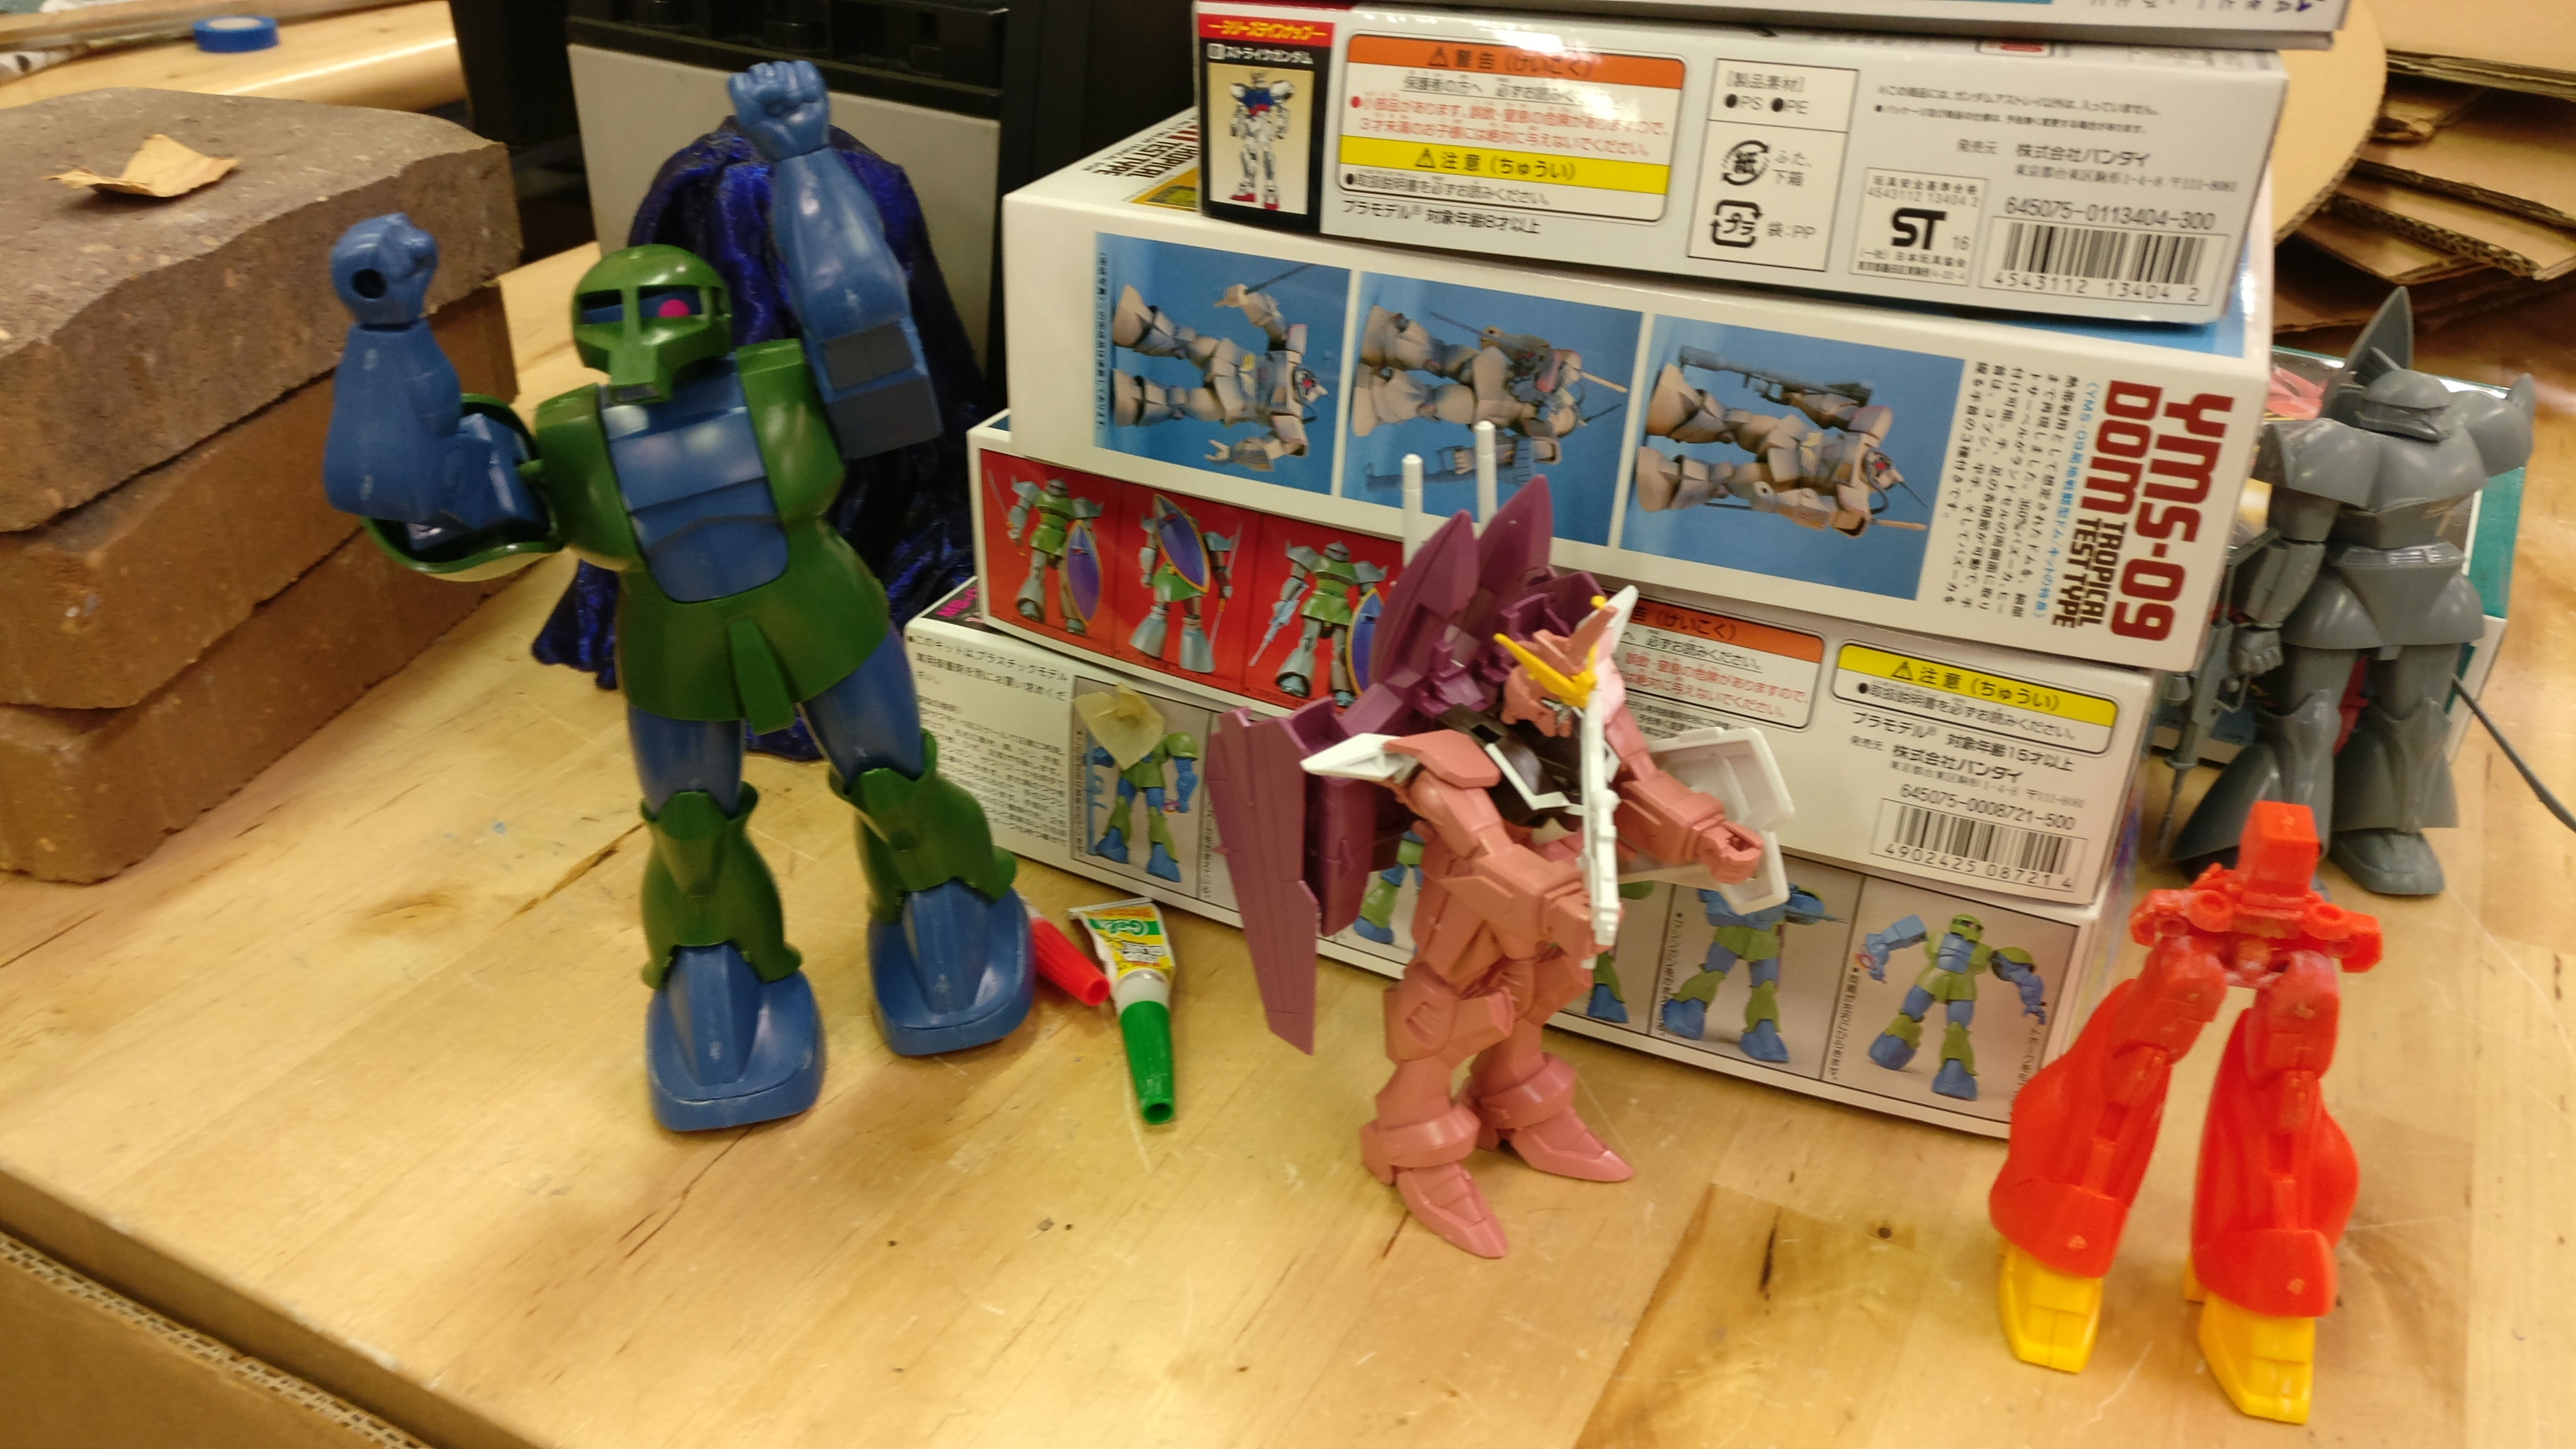
\includegraphics[width=0.3\textwidth,align=t]{../99_Bilder/00_comskill.jpg}
		\end{wrapfigure}
		In der Woche, die meiner Ankunft vorausging, haben die Schülerinnen Spielzeugmodelle zusammengebaut. Dabei hatte jede Schülerin ein eigenes Modell, aber keine Anleitung zu diesem. In der Gruppe haben die beiden anderen Mädchen nur durch verbale Kommunikation versucht, das dritte Mädchen beim Bau ihres Modells zu unterstützen. Besonders Auffällig war hier, dass die Schülerinnen für dieses Projekt gezwungen waren miteinander zu arbeiten und auf die Stärken und Schwächen ihrer Mitschüler einzugehen. Ein ähnliches Verhalten war im Verlauf der drei Wochen nicht mehr zu erkennen.\\
		Generell verlief der Unterricht sehr handlungsorientiert. Dabei hat die Lehrkraft zuvor grob erklärt, was das Ziel der Stunde ist und wie die Schülerinnen dorthin gelangen. Die Erarbeitung und die relevanten fachlichen Inhalte haben die Schülerinnen durch Recherche und Ausprobieren selbst erarbeitet.\\
		So starteten die Schüler in meiner ersten Woche mit dem Oberthema \textit{Programmieren}. Jede Schülerin war ausgestattet mit einem \textbf{Arduino Uno}, einem simplen Einplatinencomputer, sowie mit weiteren Accessoires (Kabel, Steckbrett, Sensoren und LED).\\
		\begin{center}
			\begin{tabularx}{\textwidth}{XX}
				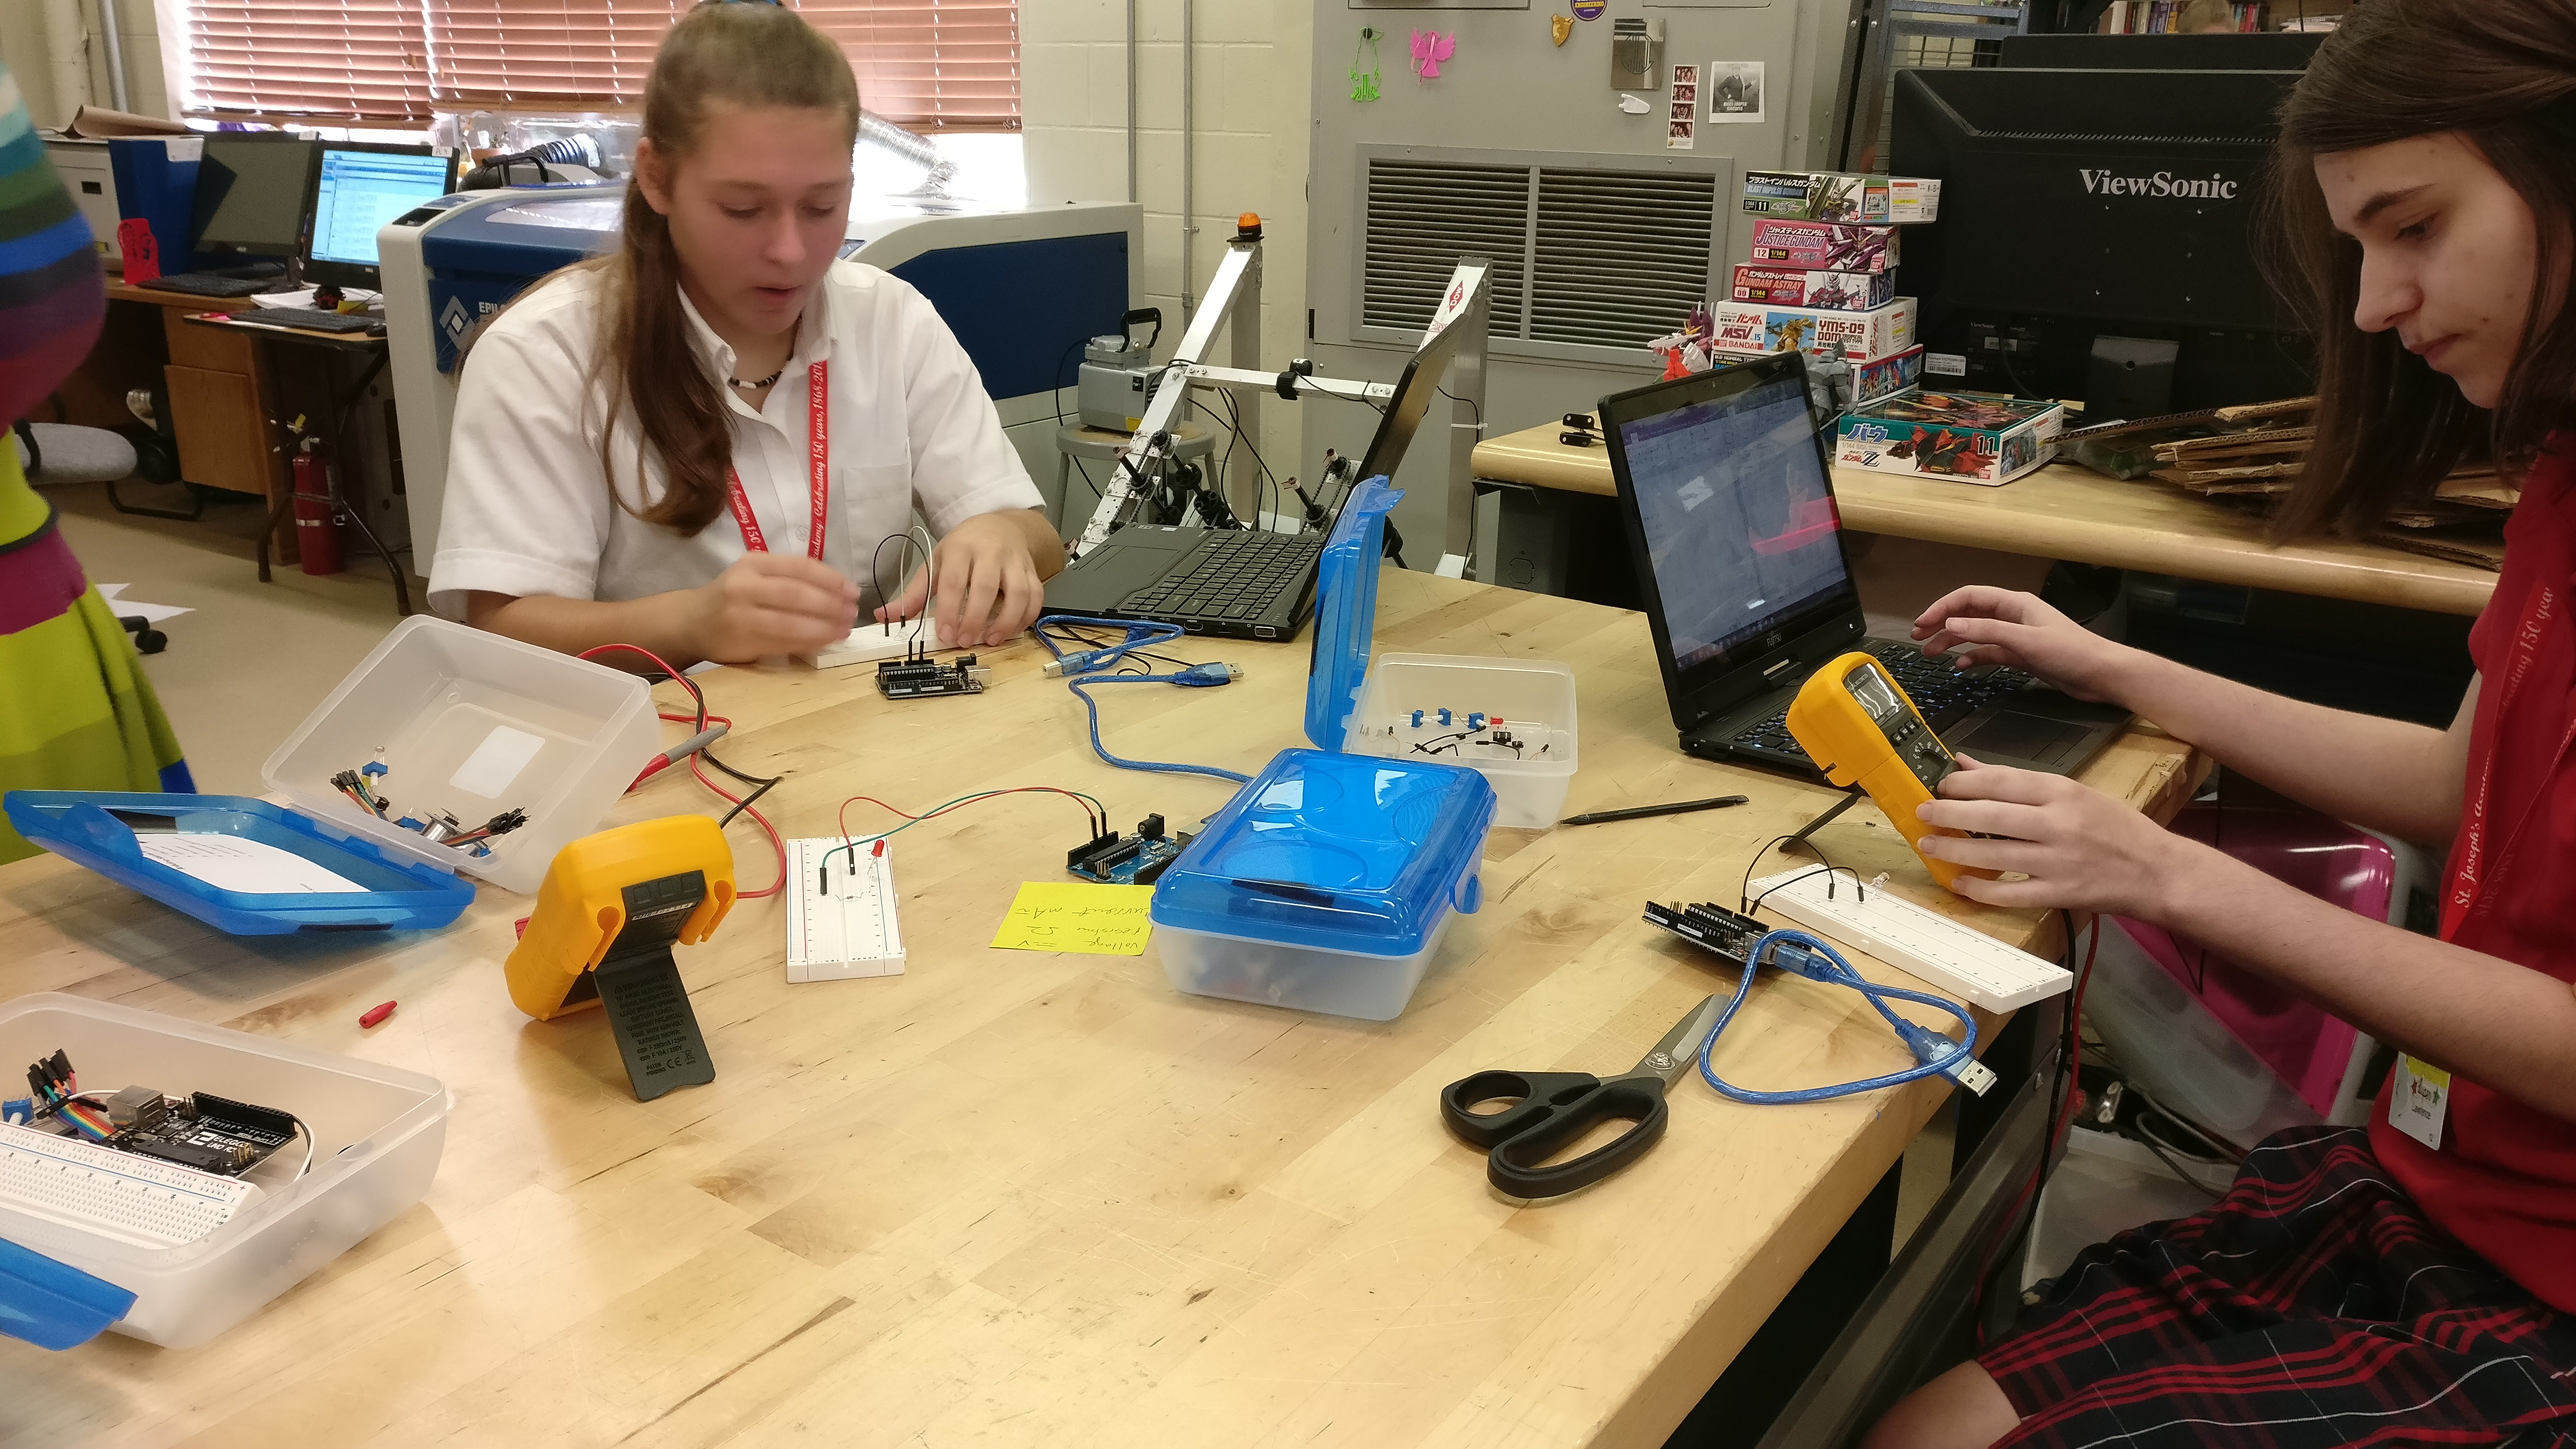
\includegraphics[width=0.48\textwidth]{../99_Bilder/00_arduino.jpg} & 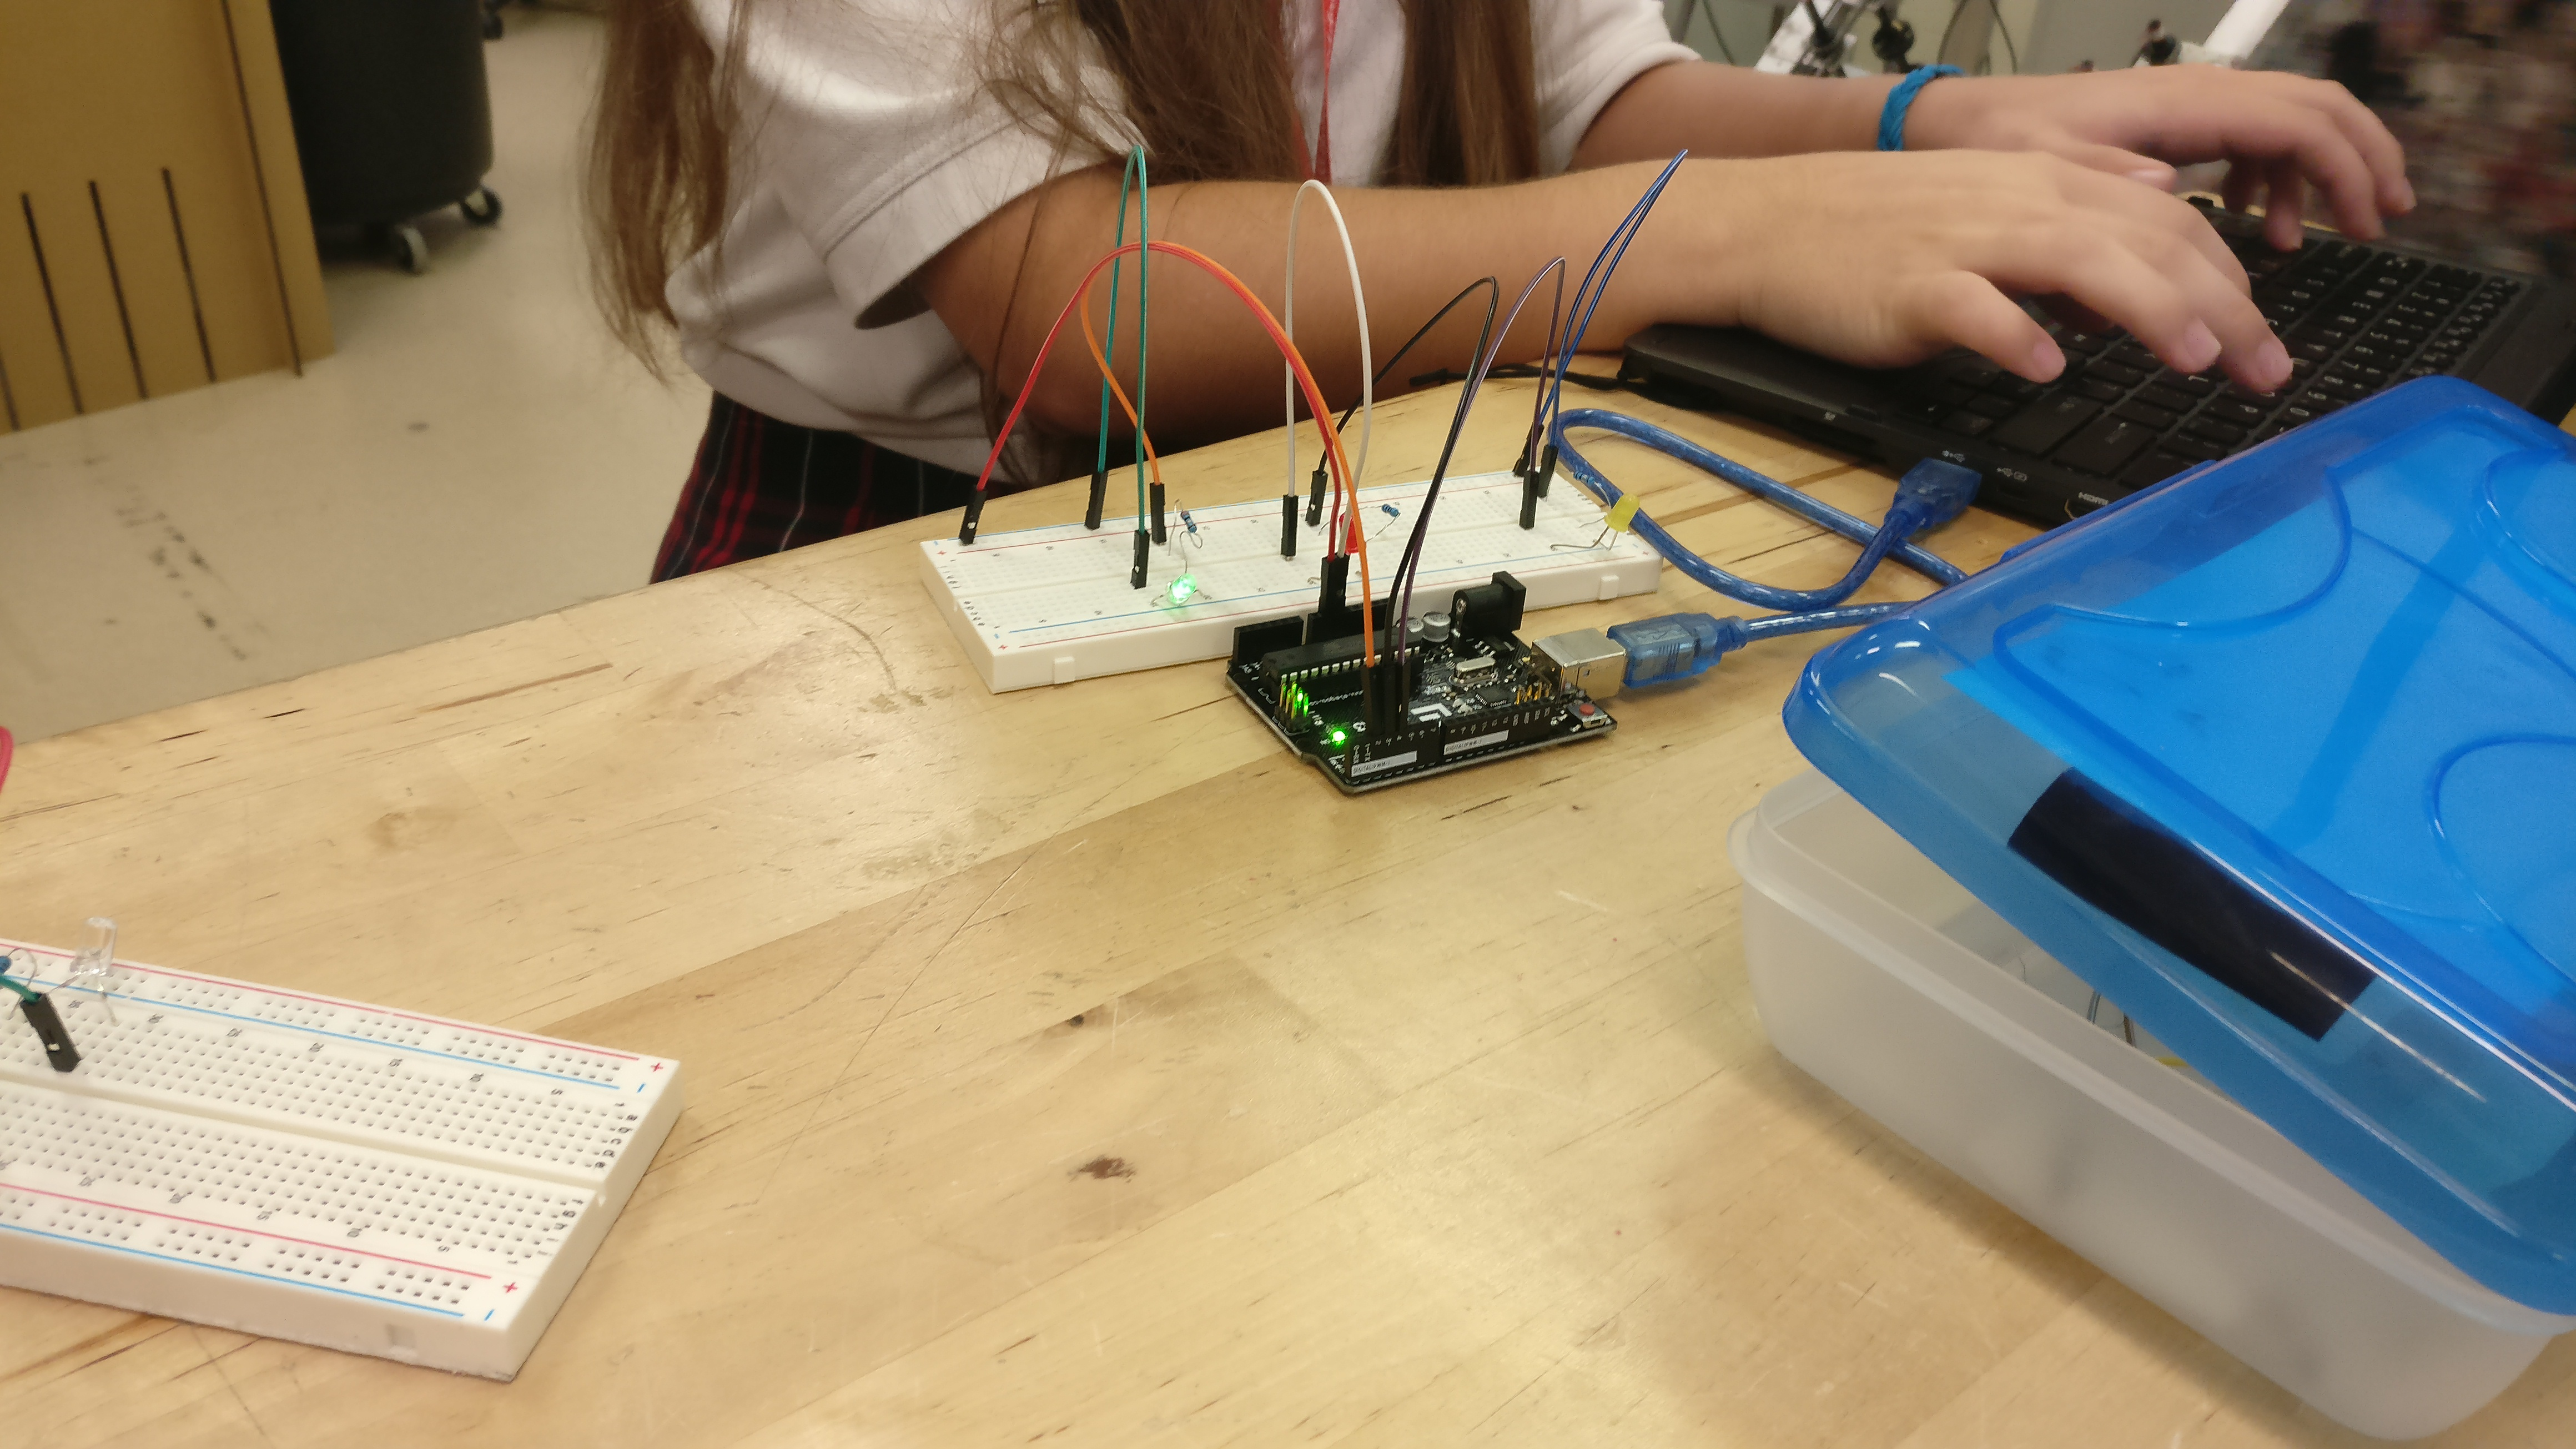
\includegraphics[width=0.48\textwidth]{../99_Bilder/01_arduino.jpg}\\
				\multicolumn{2}{c}{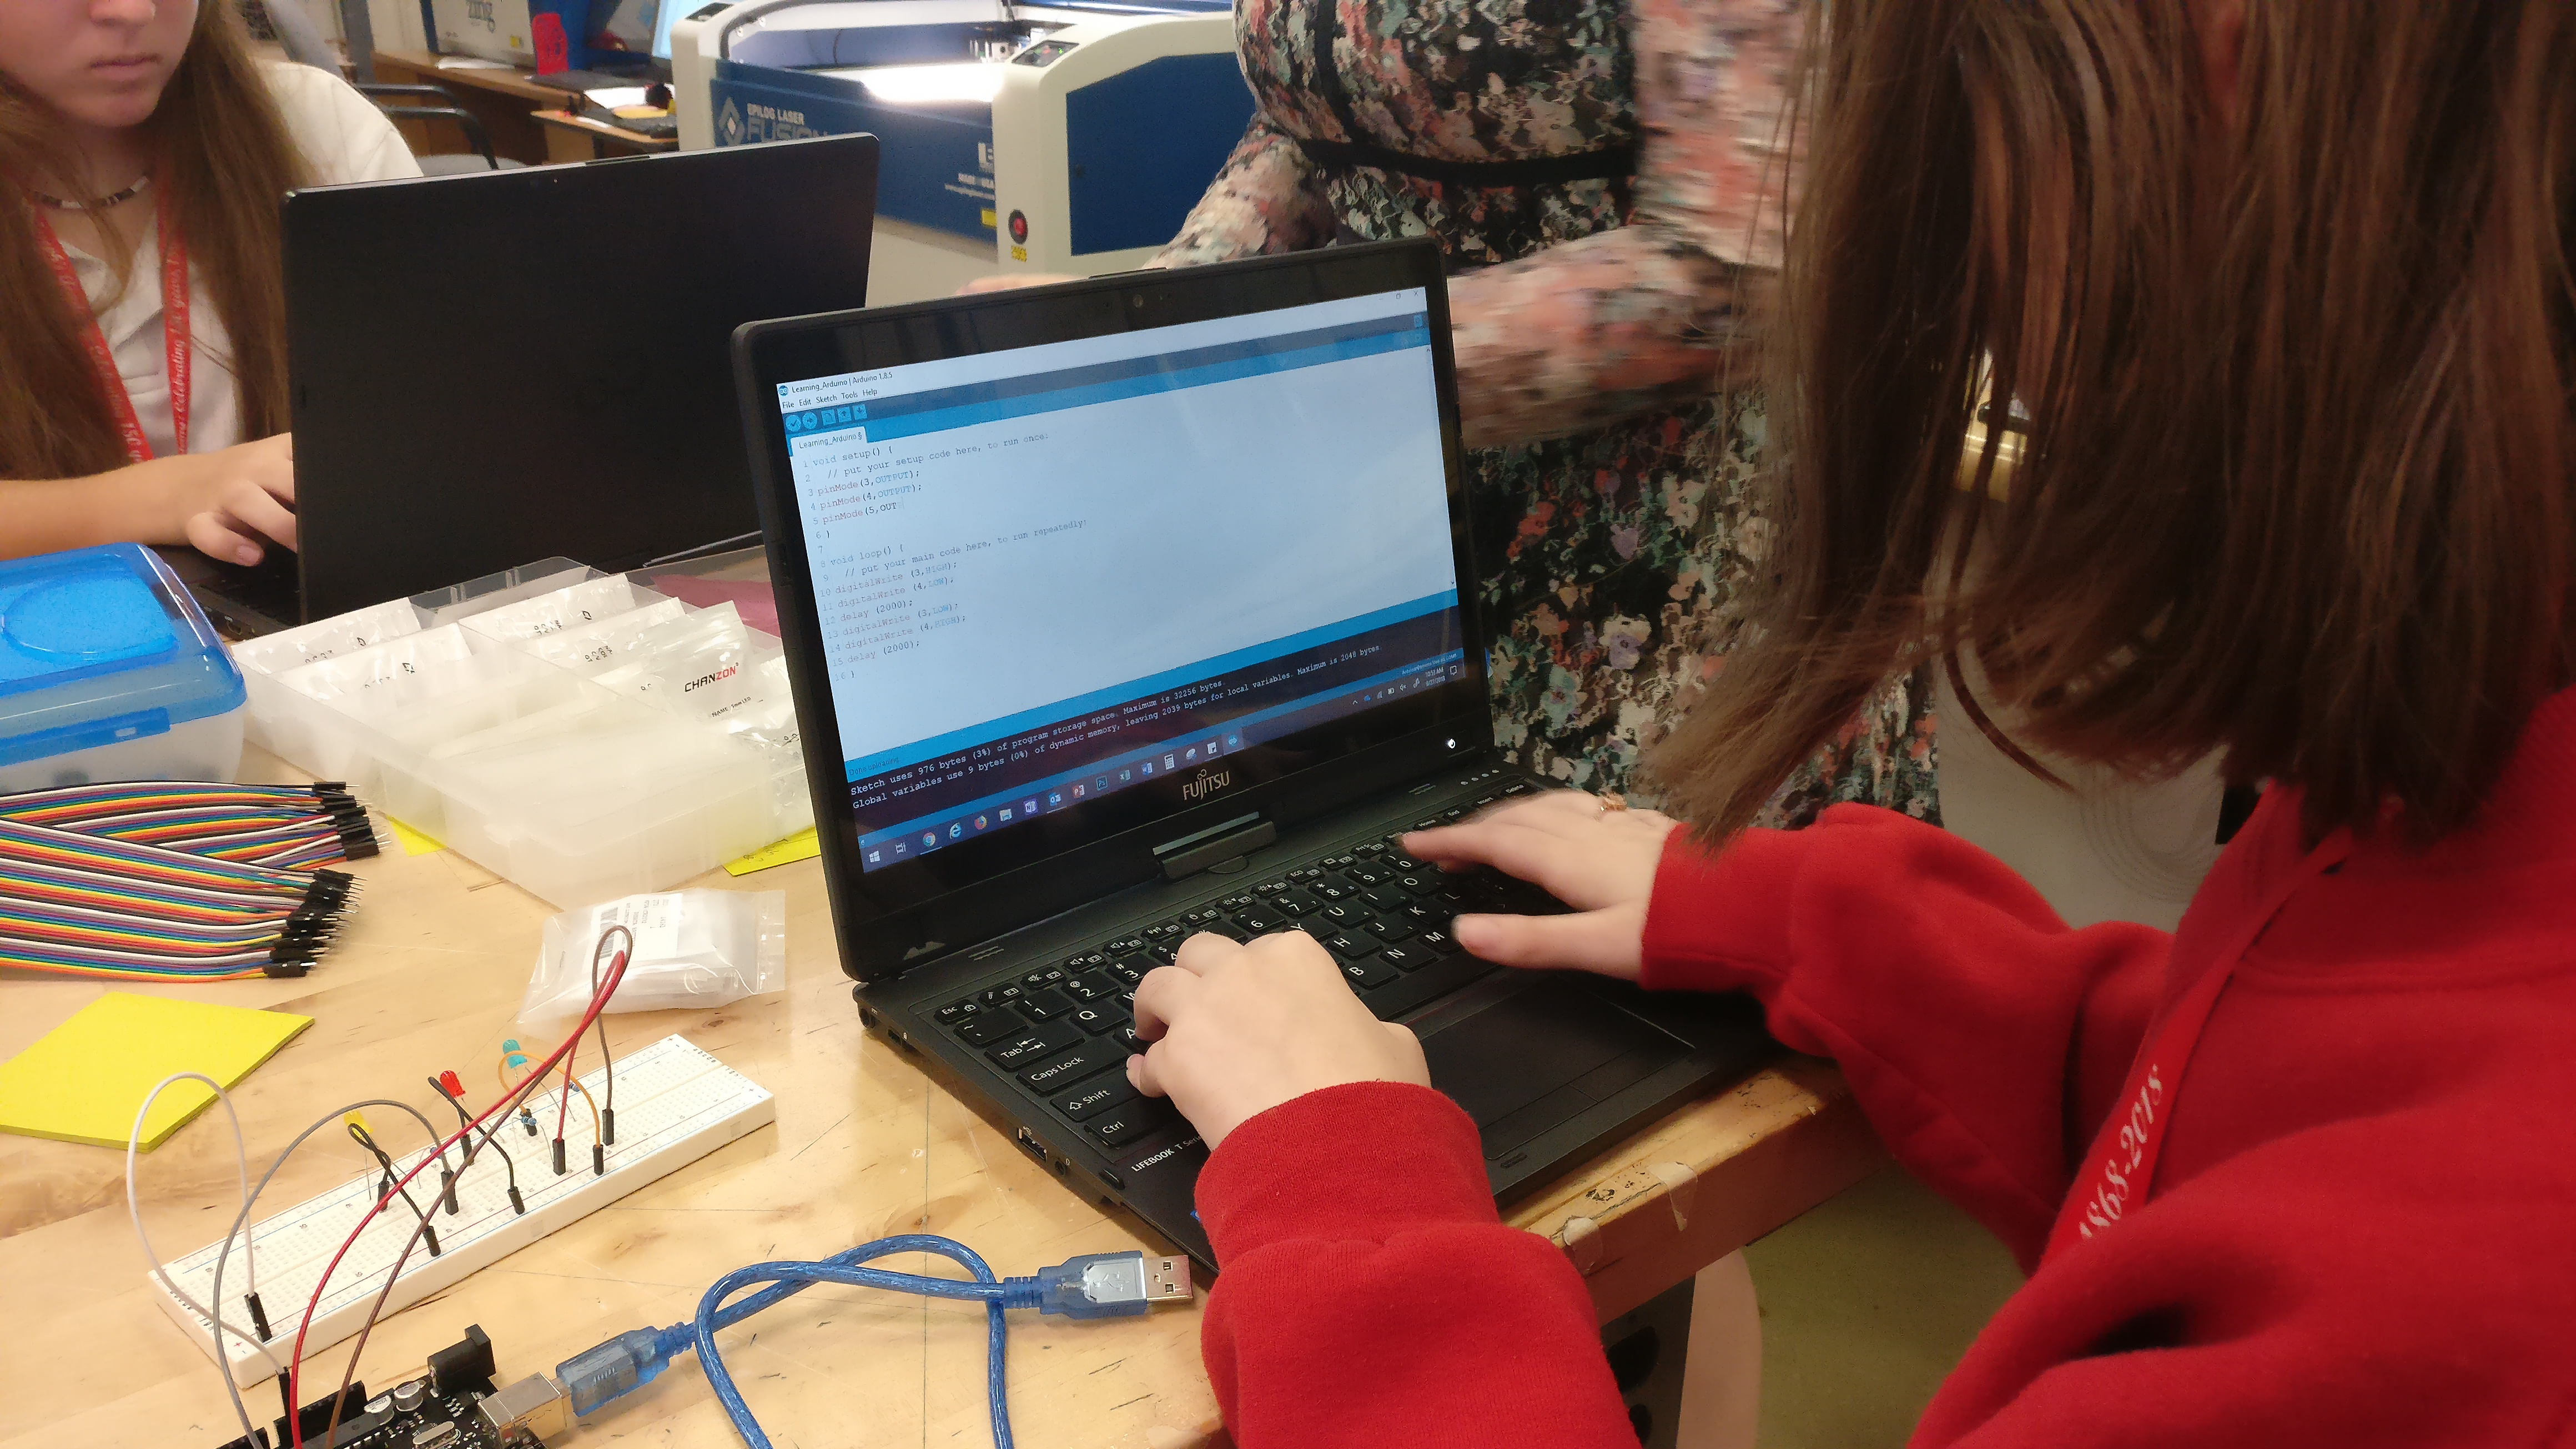
\includegraphics[width=0.48\textwidth]{../99_Bilder/02_arduino.jpg}}
			\end{tabularx}
		\end{center}
		Unabhängig von der fachlichen Ebene mussten die Schülerinnen aber während einer Unterrichtsstunde auch handwerkliche Geschicklichkeit an den Tag legen. In dieser hat die Lehrerin den Schülerinnen zunächst gezeigt, wie sie die Isolierung um ein Steckkabel abziehen und das freigelegte Kabel anschließend mit einem Lötkolben und Lötmaterial an einem Sensor befestigen.\\
		\begin{center}
			\begin{tabularx}{\textwidth}{XX}
				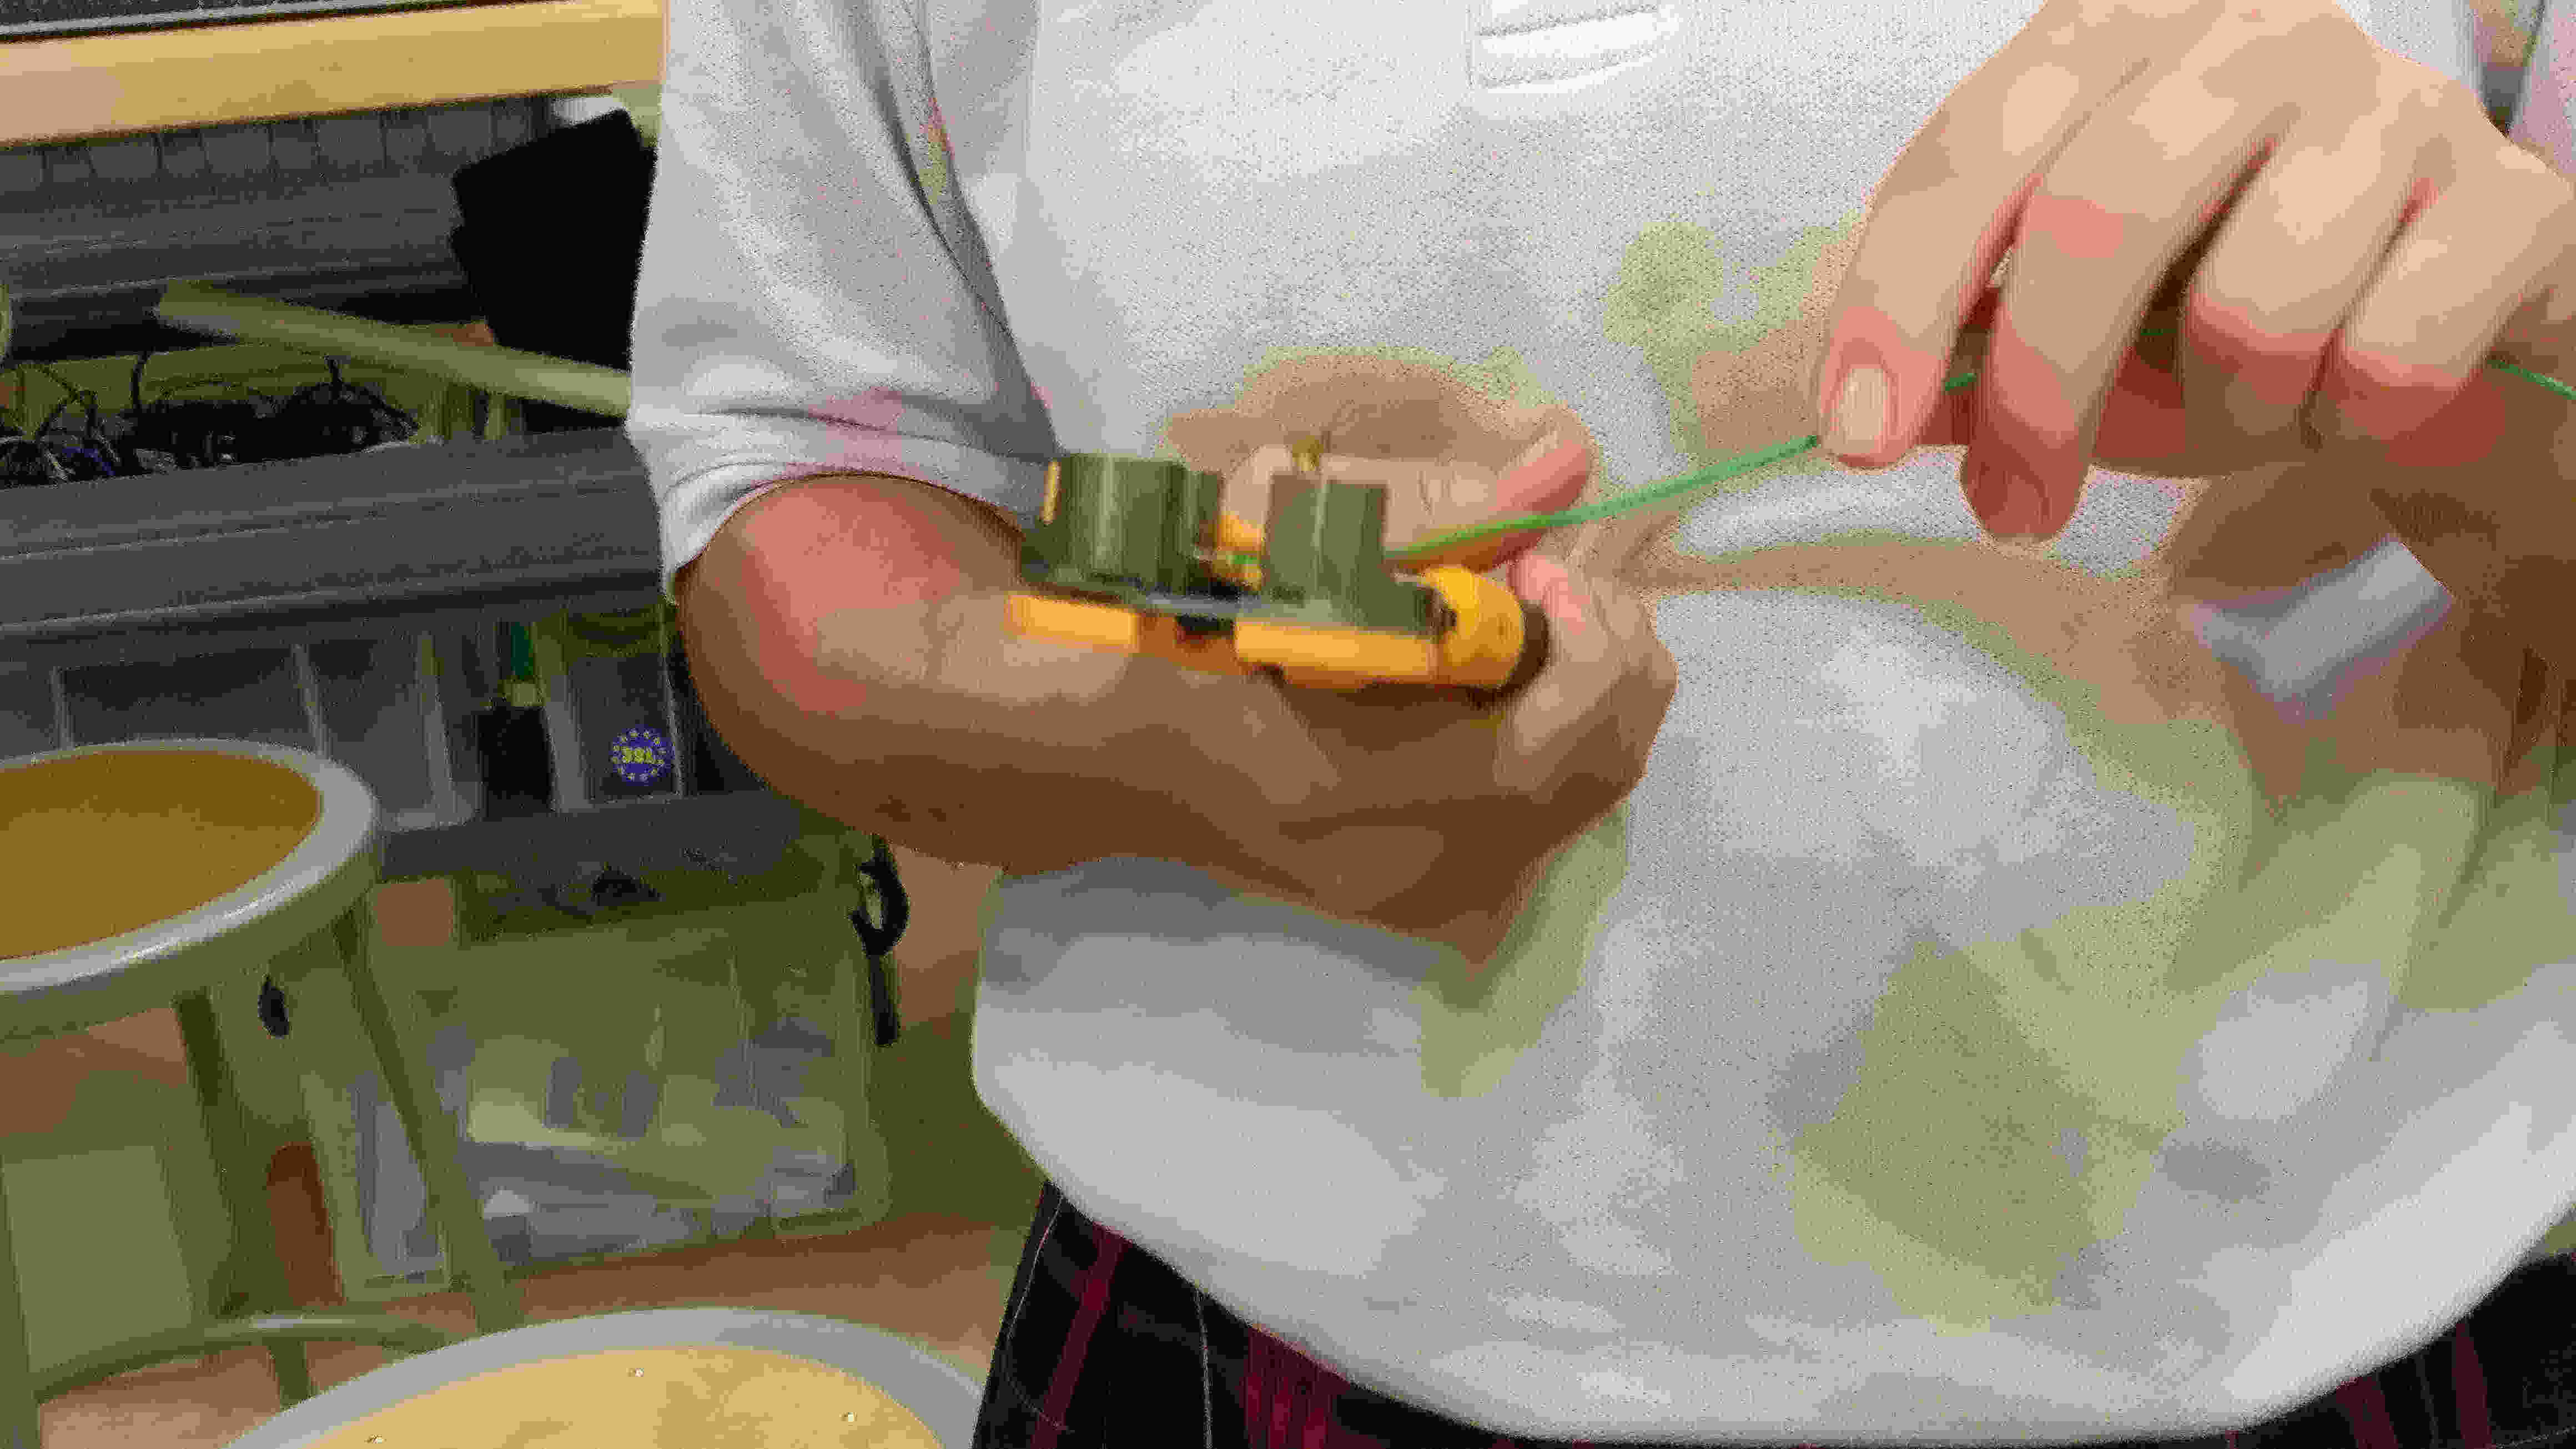
\includegraphics[width=0.48\textwidth]{../99_Bilder/00_solder.jpg} & 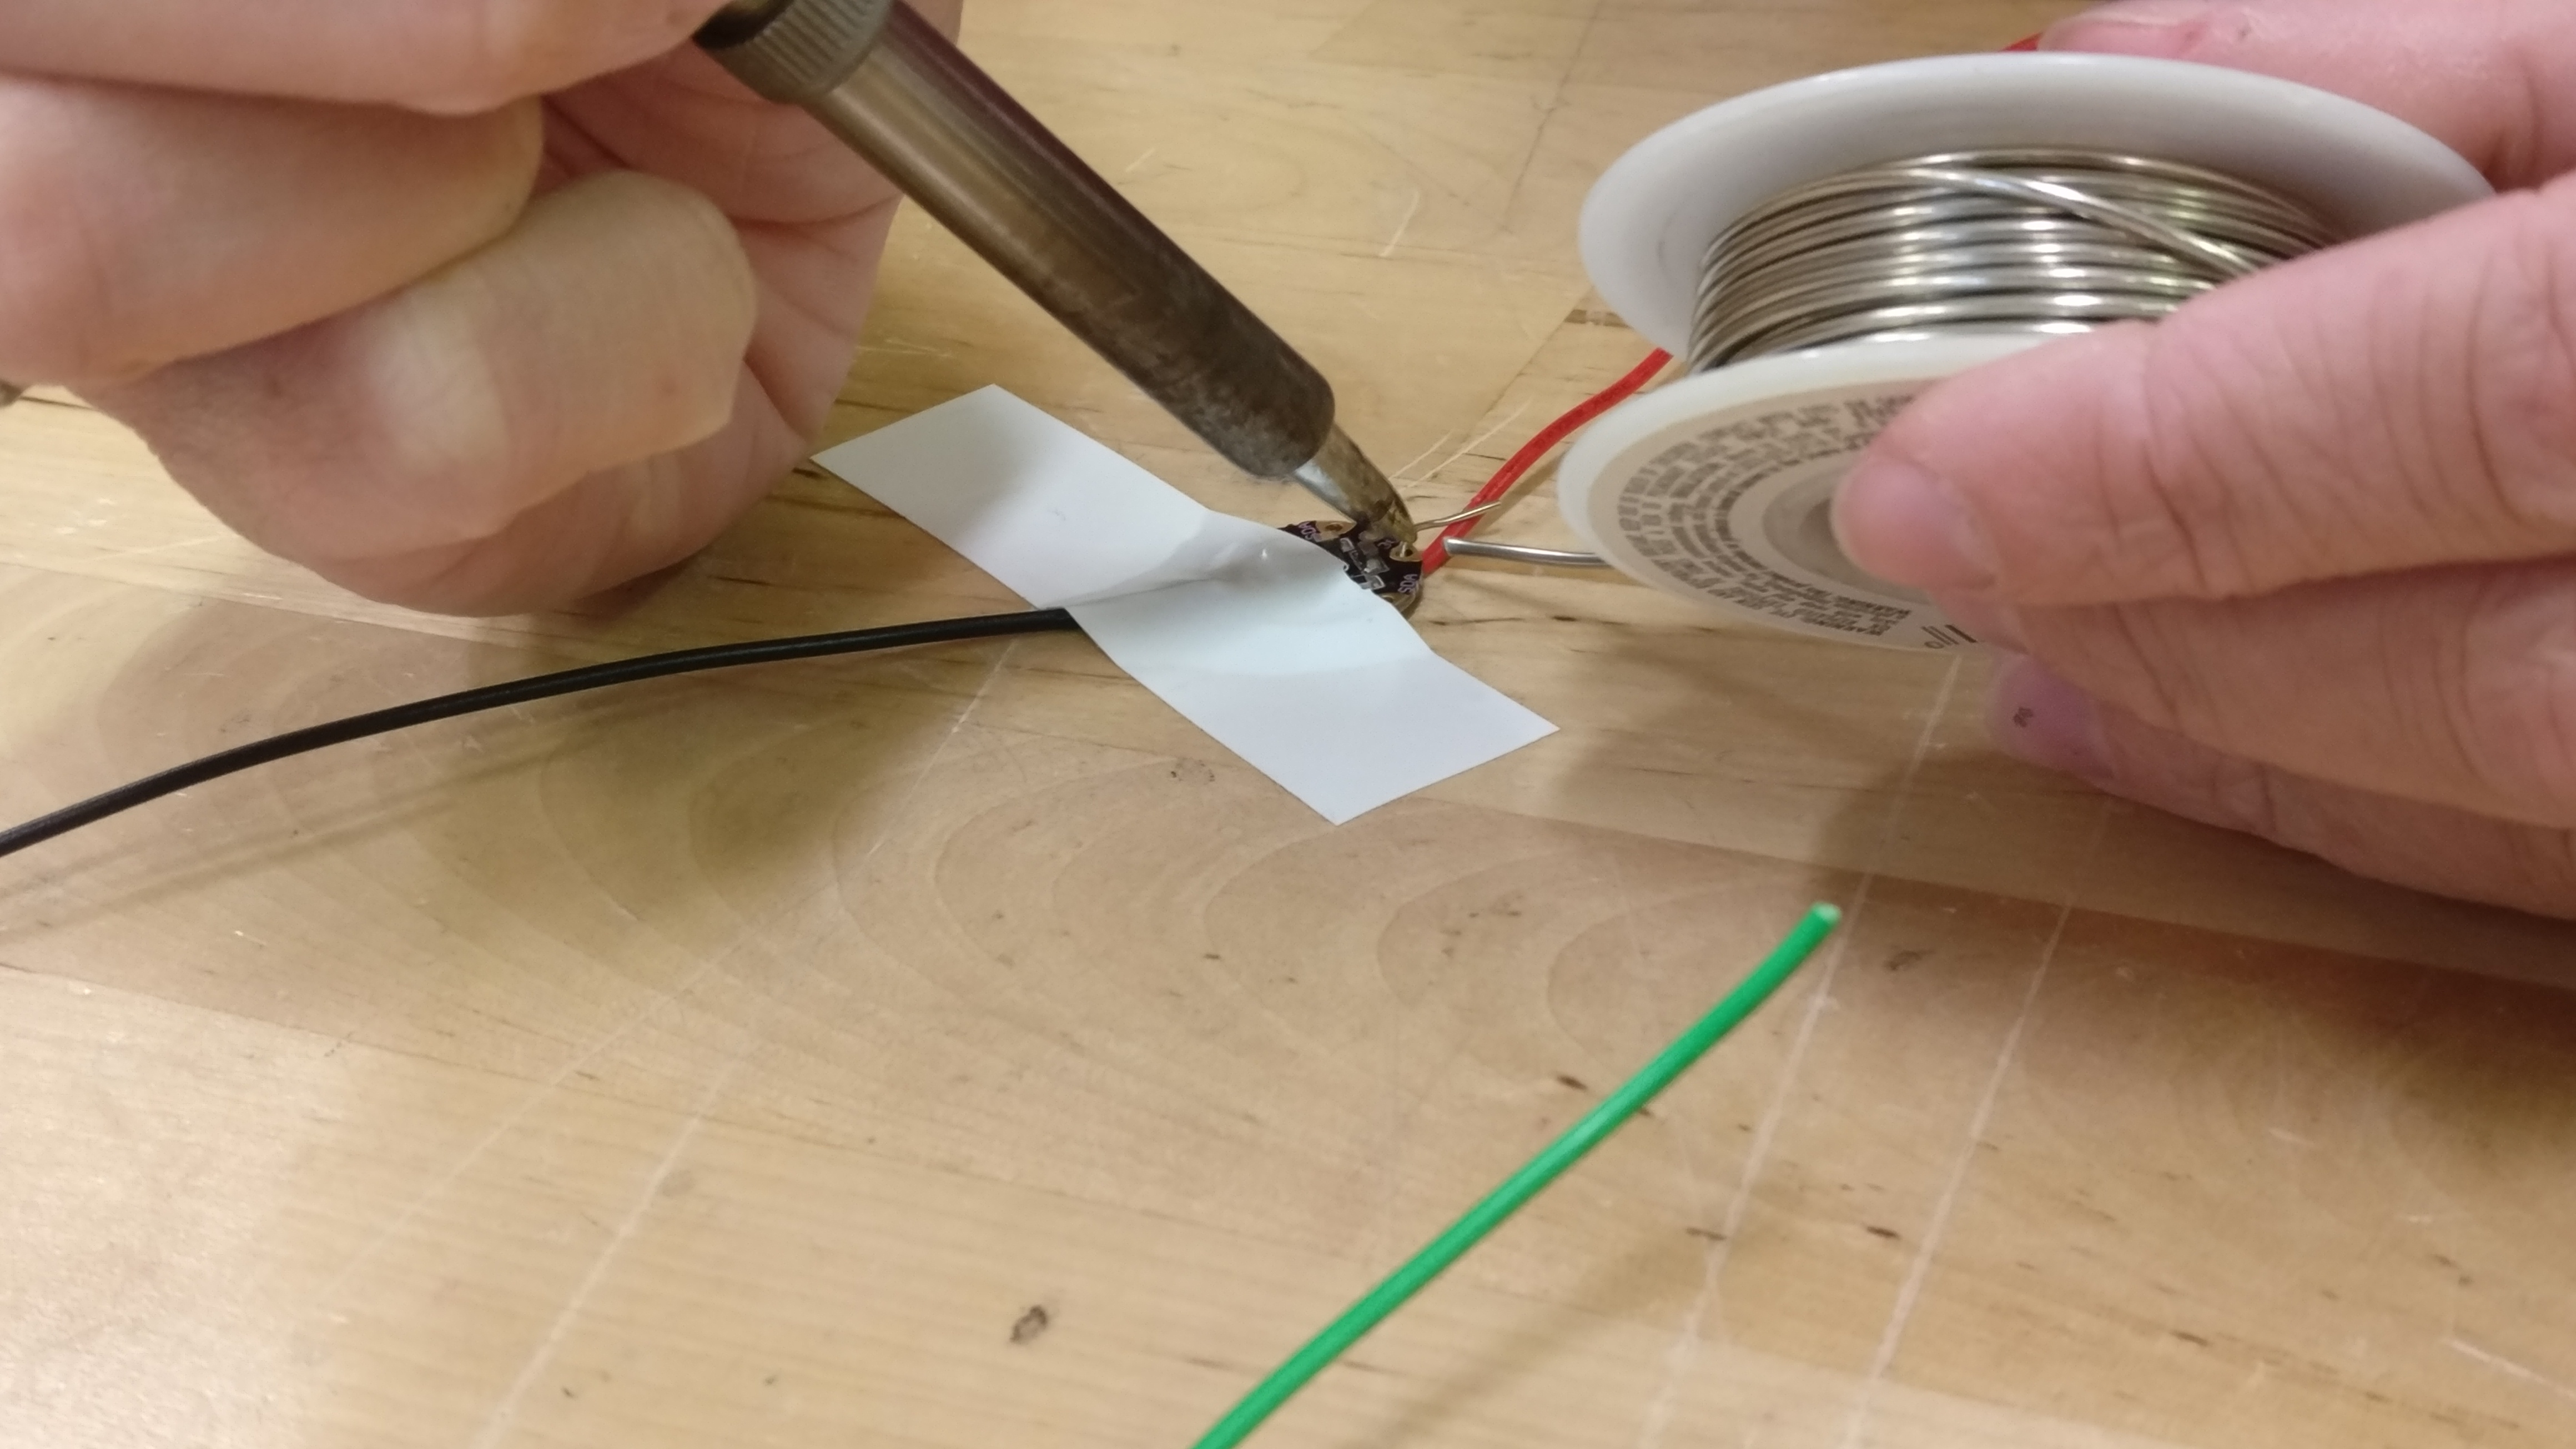
\includegraphics[width=0.48\textwidth]{../99_Bilder/01_solder.jpg}
			\end{tabularx}
		\end{center}
		Das entgegengebrachte Vertrauen wurde von den Schülerinnen entsprechend gewürdigt und sie trauten sich trotz anfänglicher Skepsis an die Aufgabe des Lötens heran.\\
		Im Gegensatz zu anderen Unterrichtsstunden, in denen die Schüler eher lethargisch auf ihren Plätzen saßen, haben die Schülerinnen im STEM-Lab aktiv und engagiert am Unterricht teilgenommen und selbstständig ohne große Instruktion gearbeitet.\\
		\par\noindent
		Ein weiteres Projekt, das die Schülerinnen über einen längeren Zeitraum während der STEM-Lab Stunde verfolgen ist der Bau eines Stuhls aus Pappe.\\Als Material dient den Schülerinnen dicke Verpackungspappe. Die einzelnen Stuhlelemente werden anhand einer Schablone von dem zur Verfügung stehenden Laserdrucker geschnitten.\\
		Damit die Pappe in den Laserdrucker passt, müssen die Schülerinnen sie ausmessen und mit einem Teppichmesser zurecht schneiden in die korrekte Größe bringen. Besonders bei der Handhabung des Teppichmesser wird den Schülerinnen viel Vertrauen entgegengebracht.\\
		Sie arbeiten entsprechend gewissenhaft und achten immer auf eine korrekte Handhabung und Verstauung des Teppichmesser.
		\begin{center}
			\begin{tabularx}{\textwidth}{XX}
				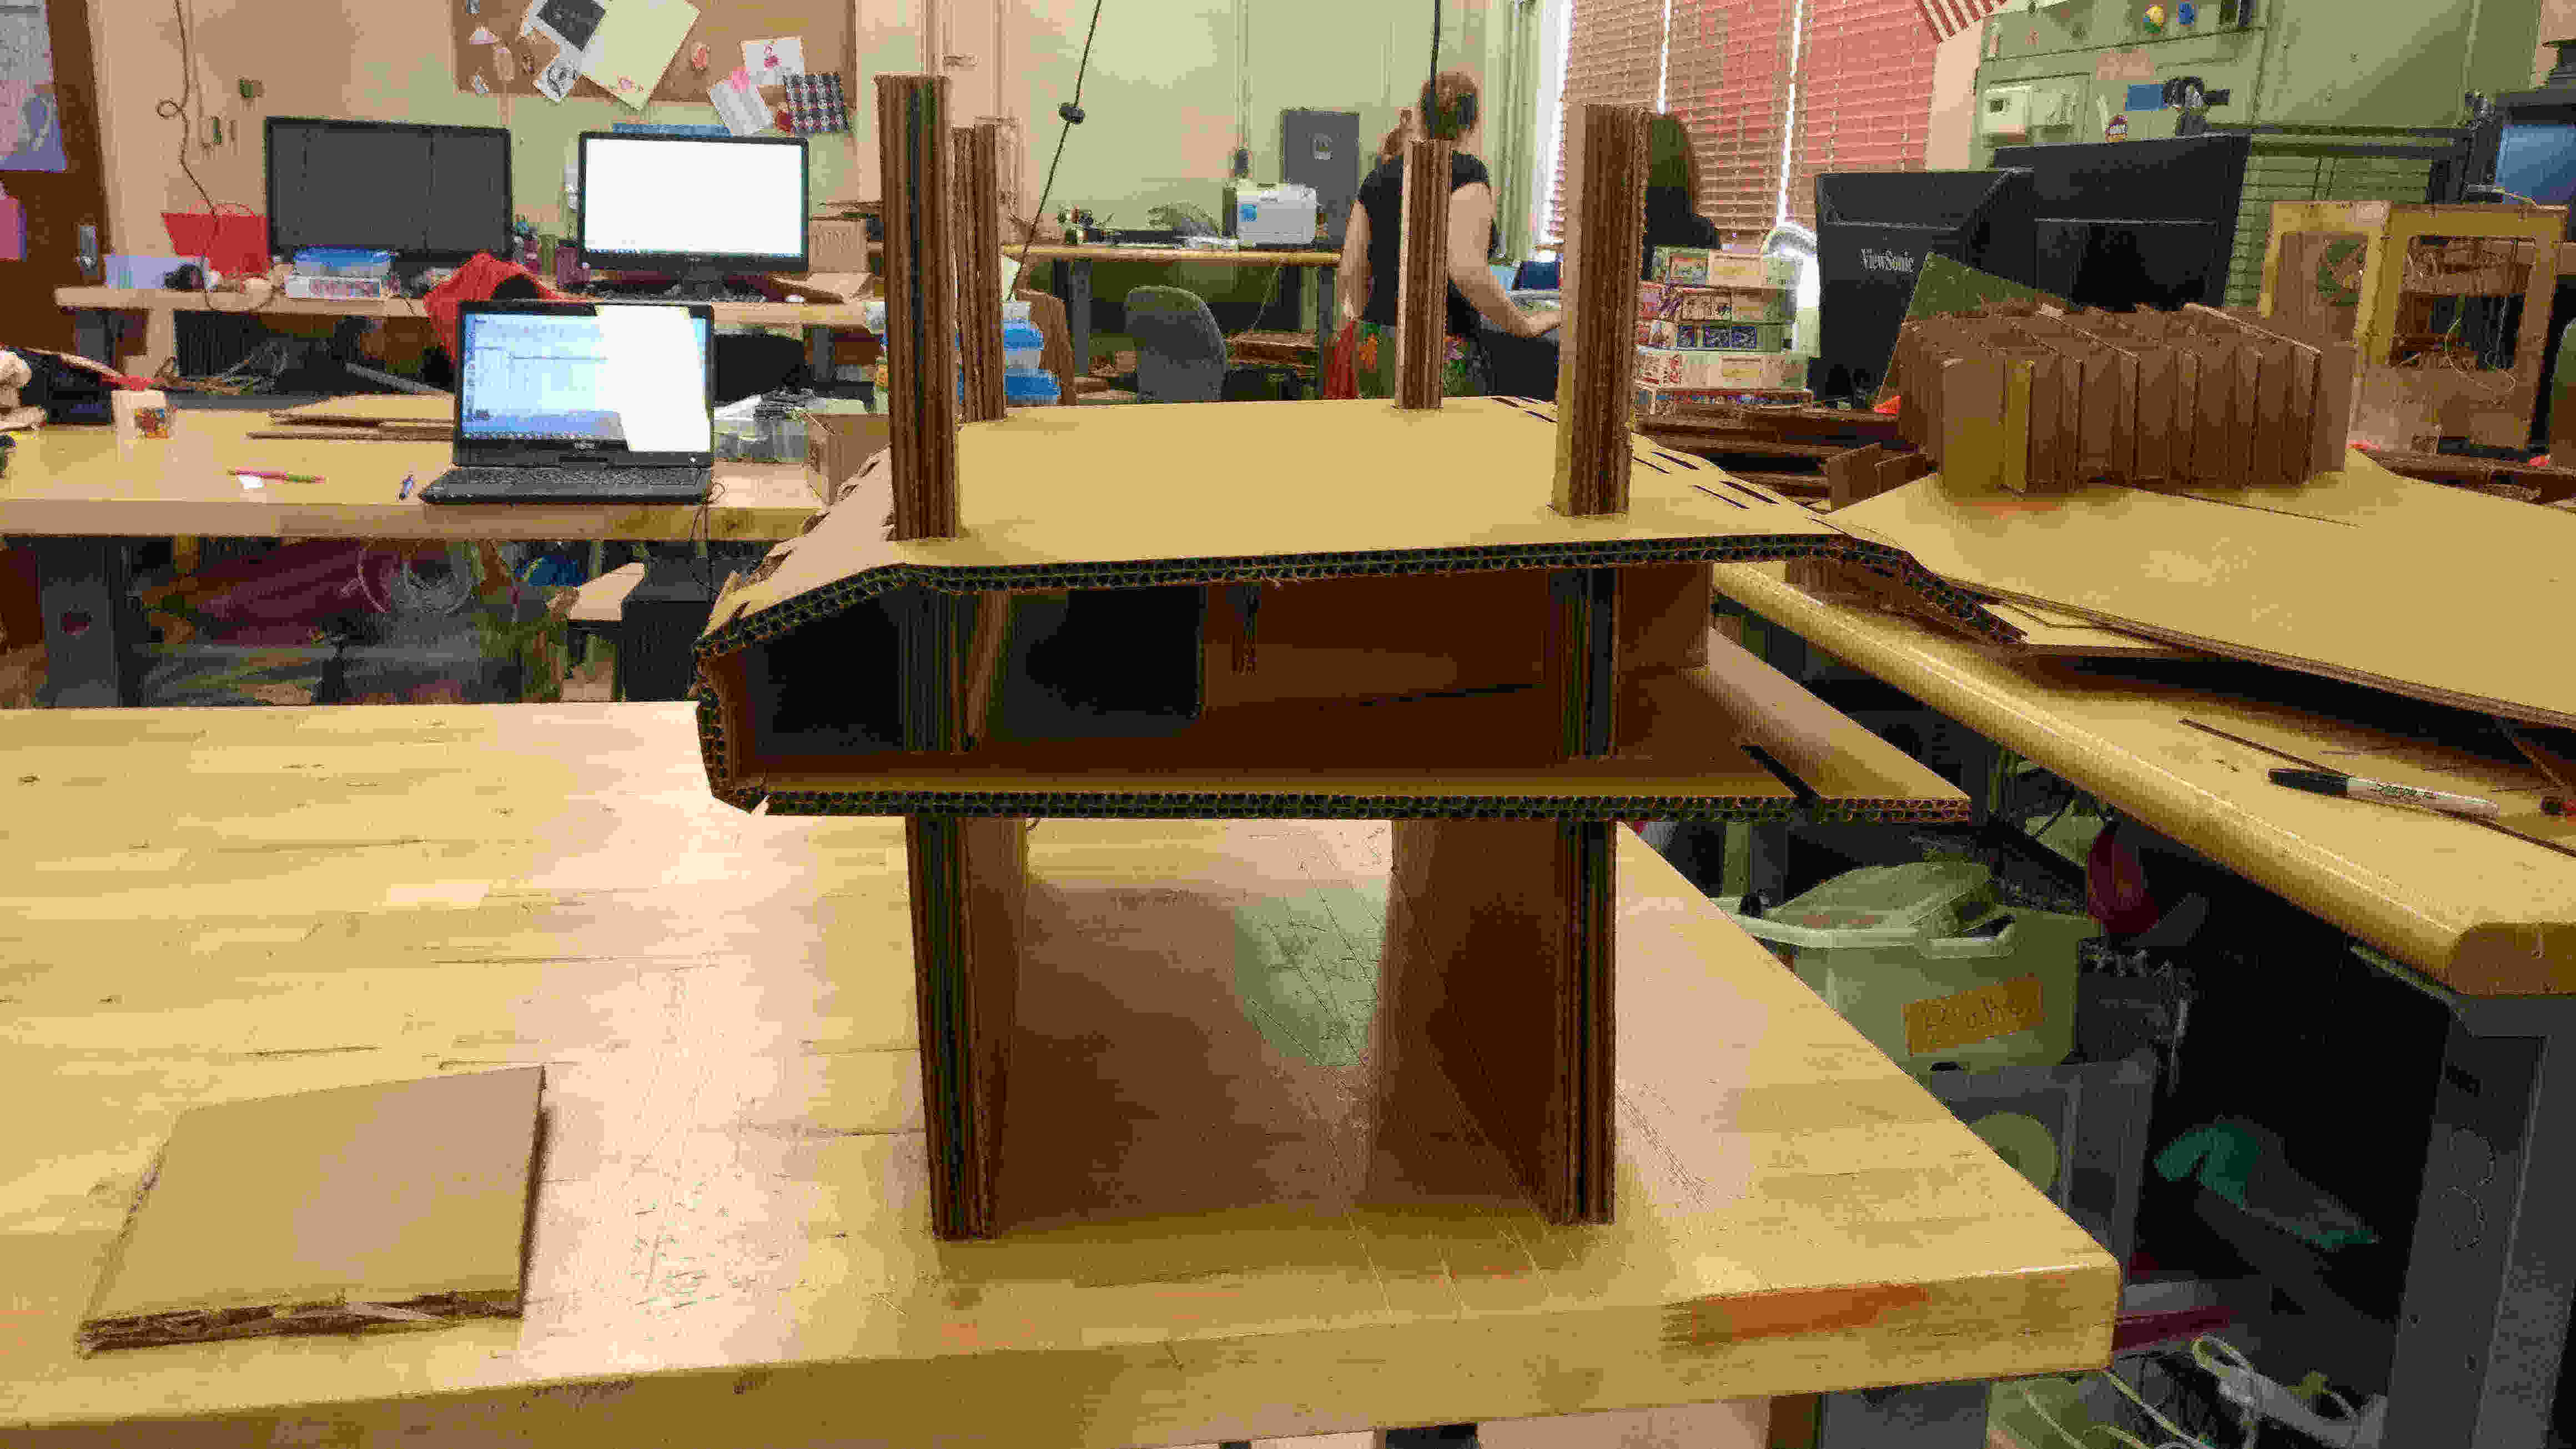
\includegraphics[width=0.48\textwidth,align=t]{../99_Bilder/00_chair.jpg} & 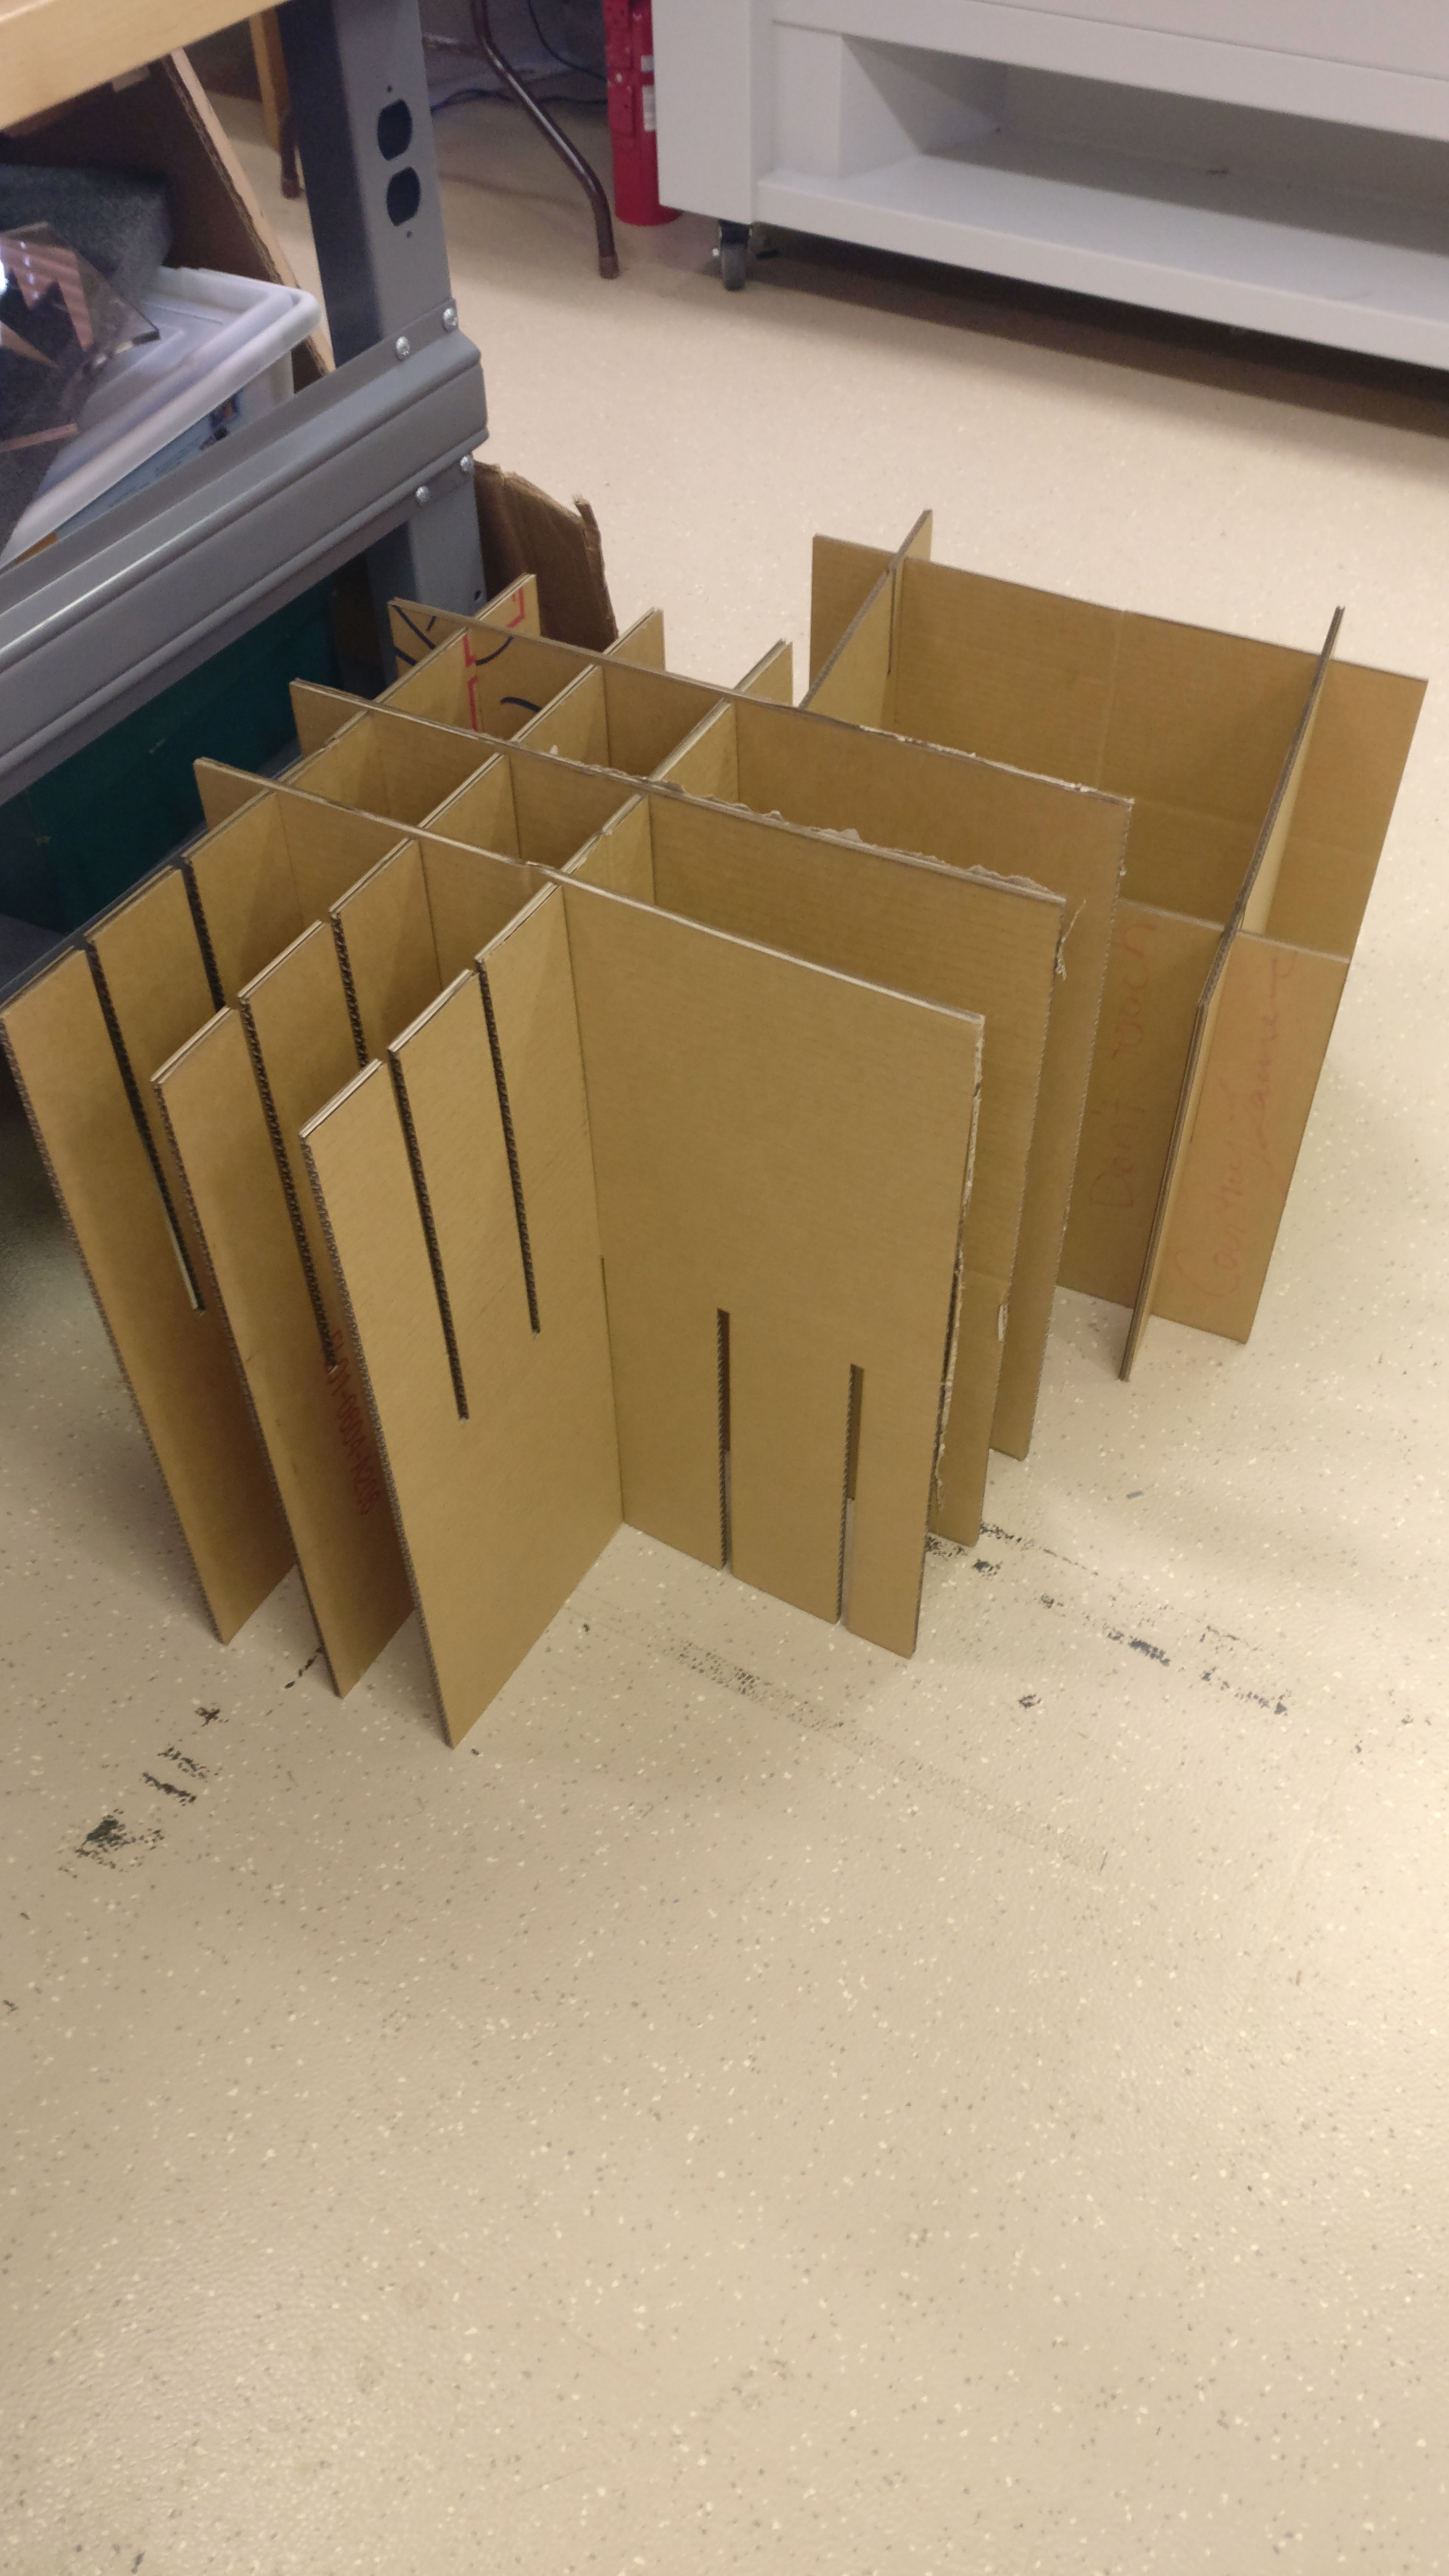
\includegraphics[width=0.48\textwidth,align=t]{../99_Bilder/01_chair.jpg}
			\end{tabularx}
			\begin{tabularx}{\textwidth}{XX}
				
\includegraphics[width=0.48\textwidth]{../99_Bilder/00_laser.jpg} & 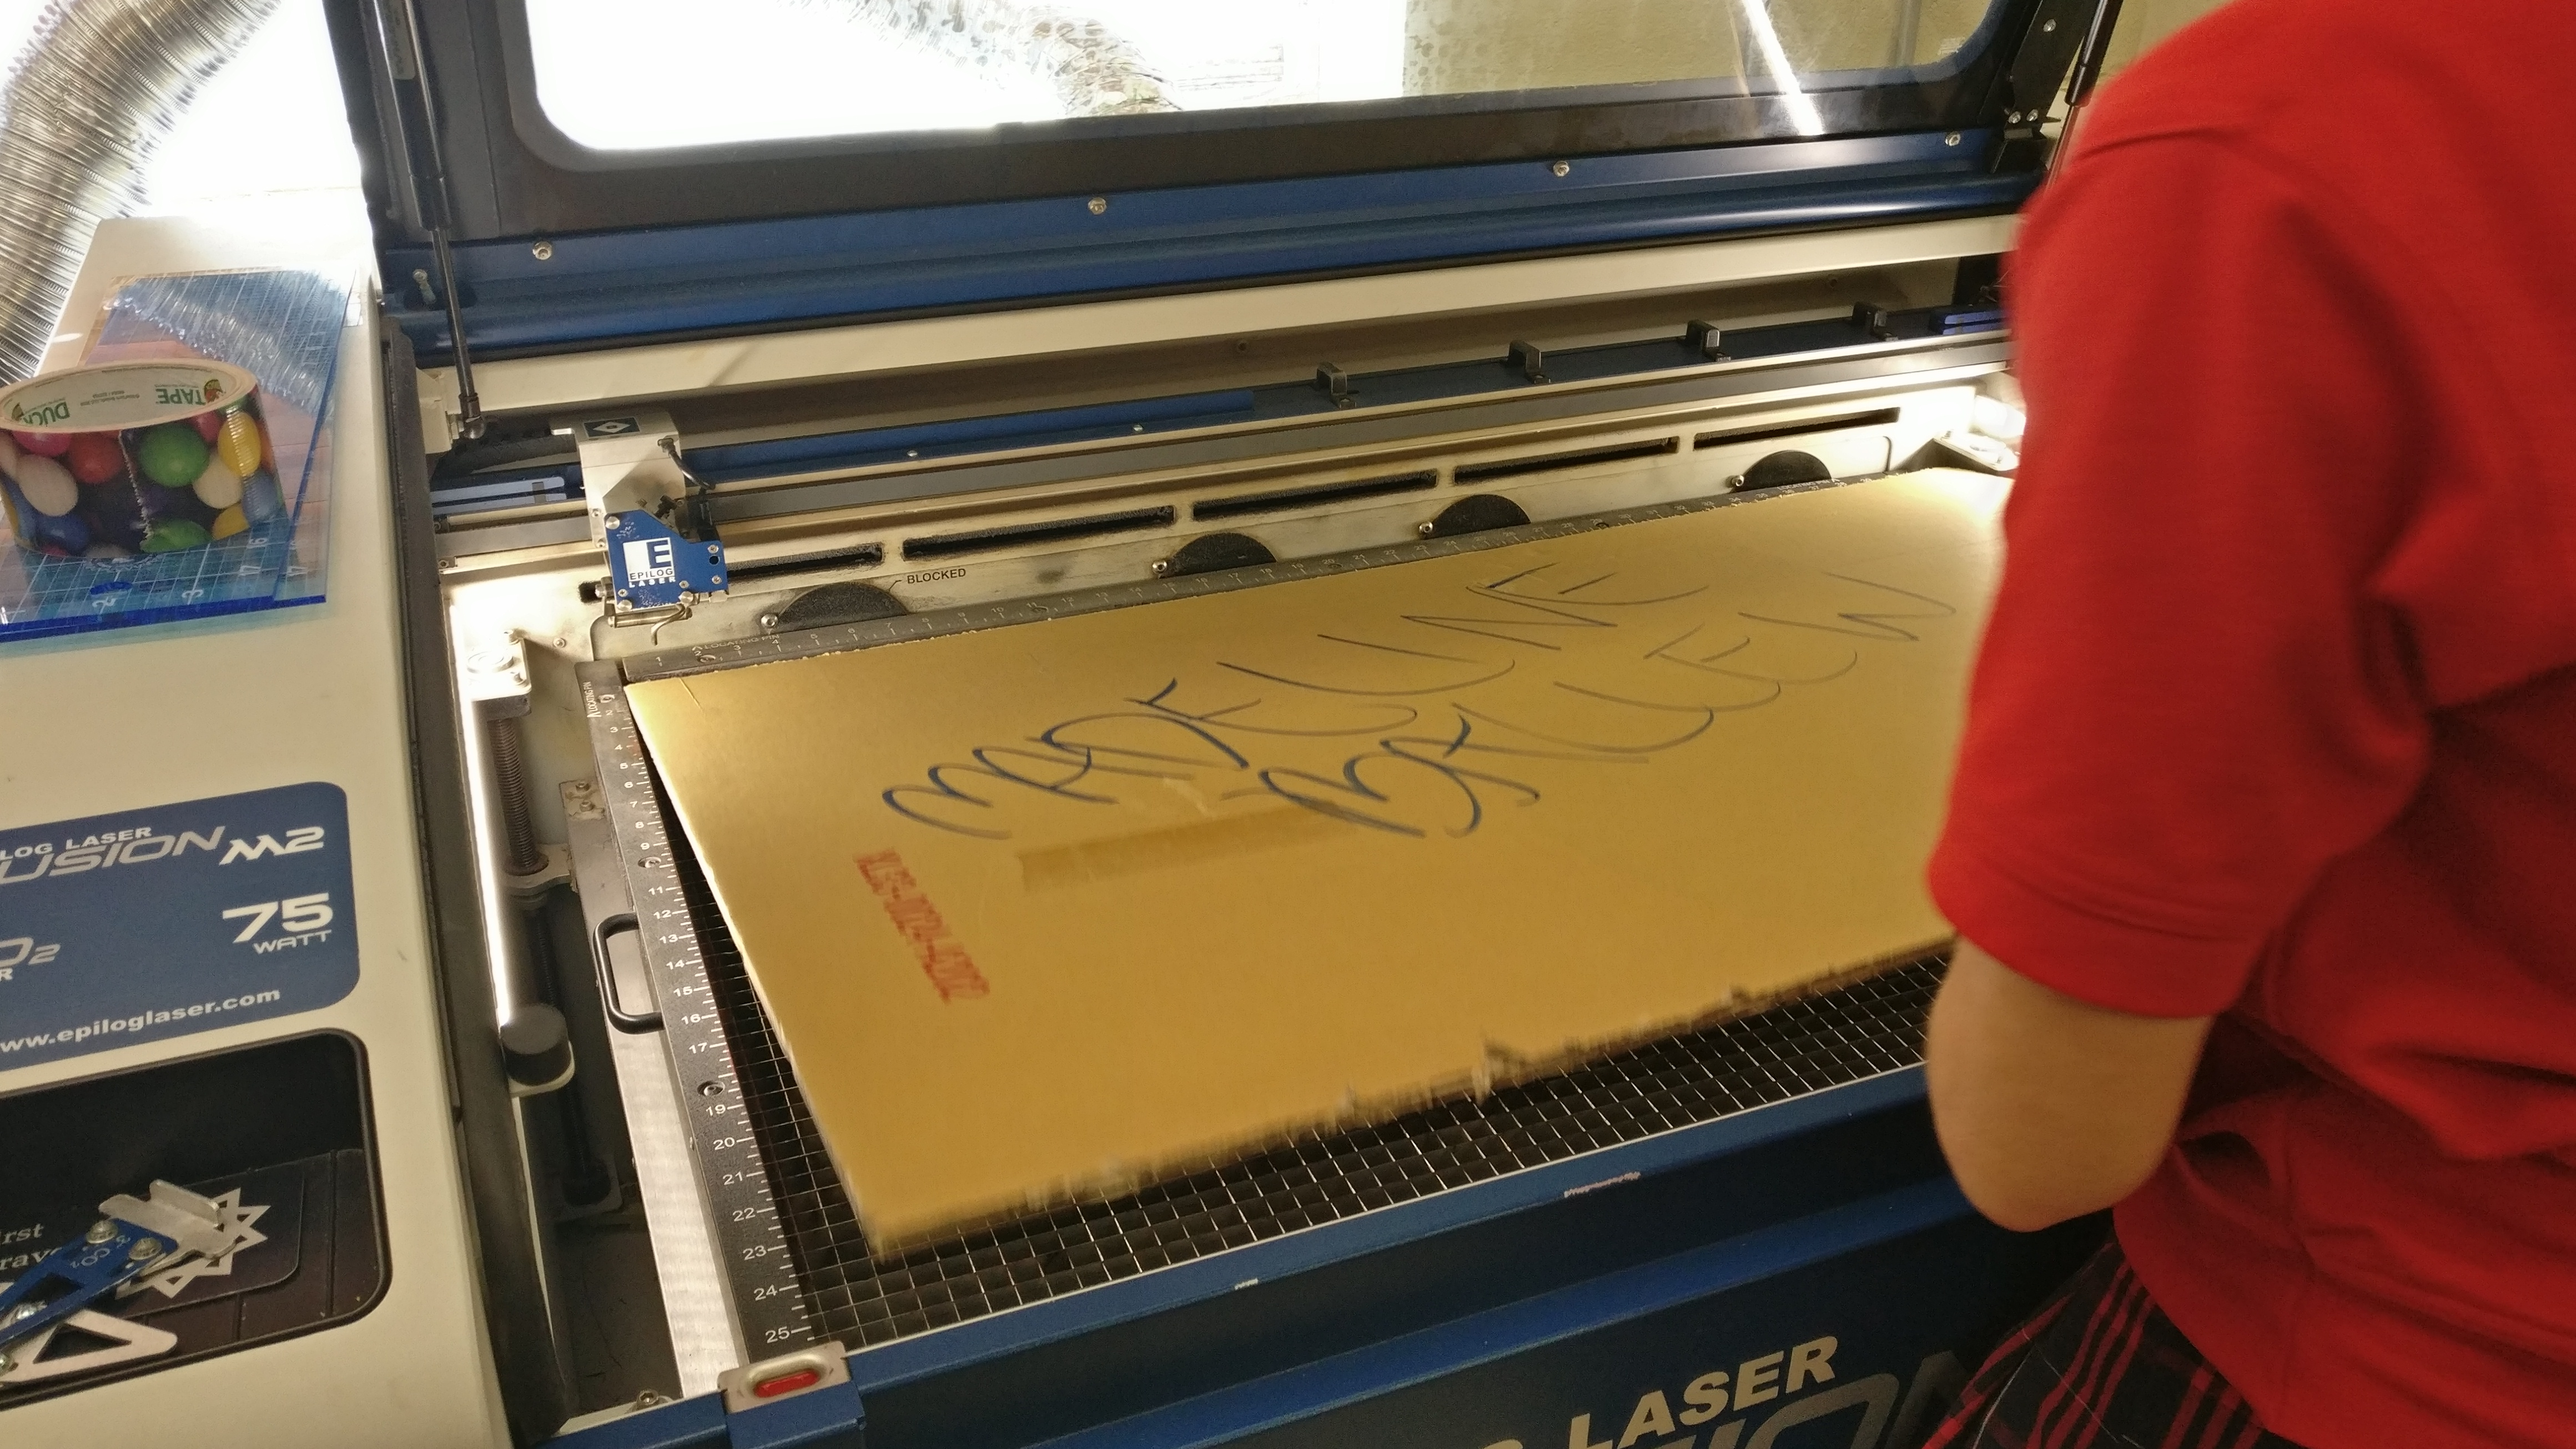
\includegraphics[width=0.48\textwidth]{../99_Bilder/01_laser.jpg}
			\end{tabularx}
		\end{center}
		Die Möglichkeit den Laserdrucker wie auch der im STEM-Lab zur Verfügung stehende 3D-Drucker zu nutzen, findet in den anderen Abteilung großen Anklang, sodass die im STEM-Lab angestellten Lehrkräfte auch \grq{}fachfremdes\grq{} produzieren.\\
		Hierfür gehen die STEM-Lehrkräfte in die Kurse, in denen die Gerätschaften genutzt werden sollen und informieren die Schülerinnen über die Handhabung, Funktionalität und Vorgehensweise die bei der Nutzung zu beachten ist.
		\begin{center}
			\begin{tabularx}{\textwidth}{XX}
				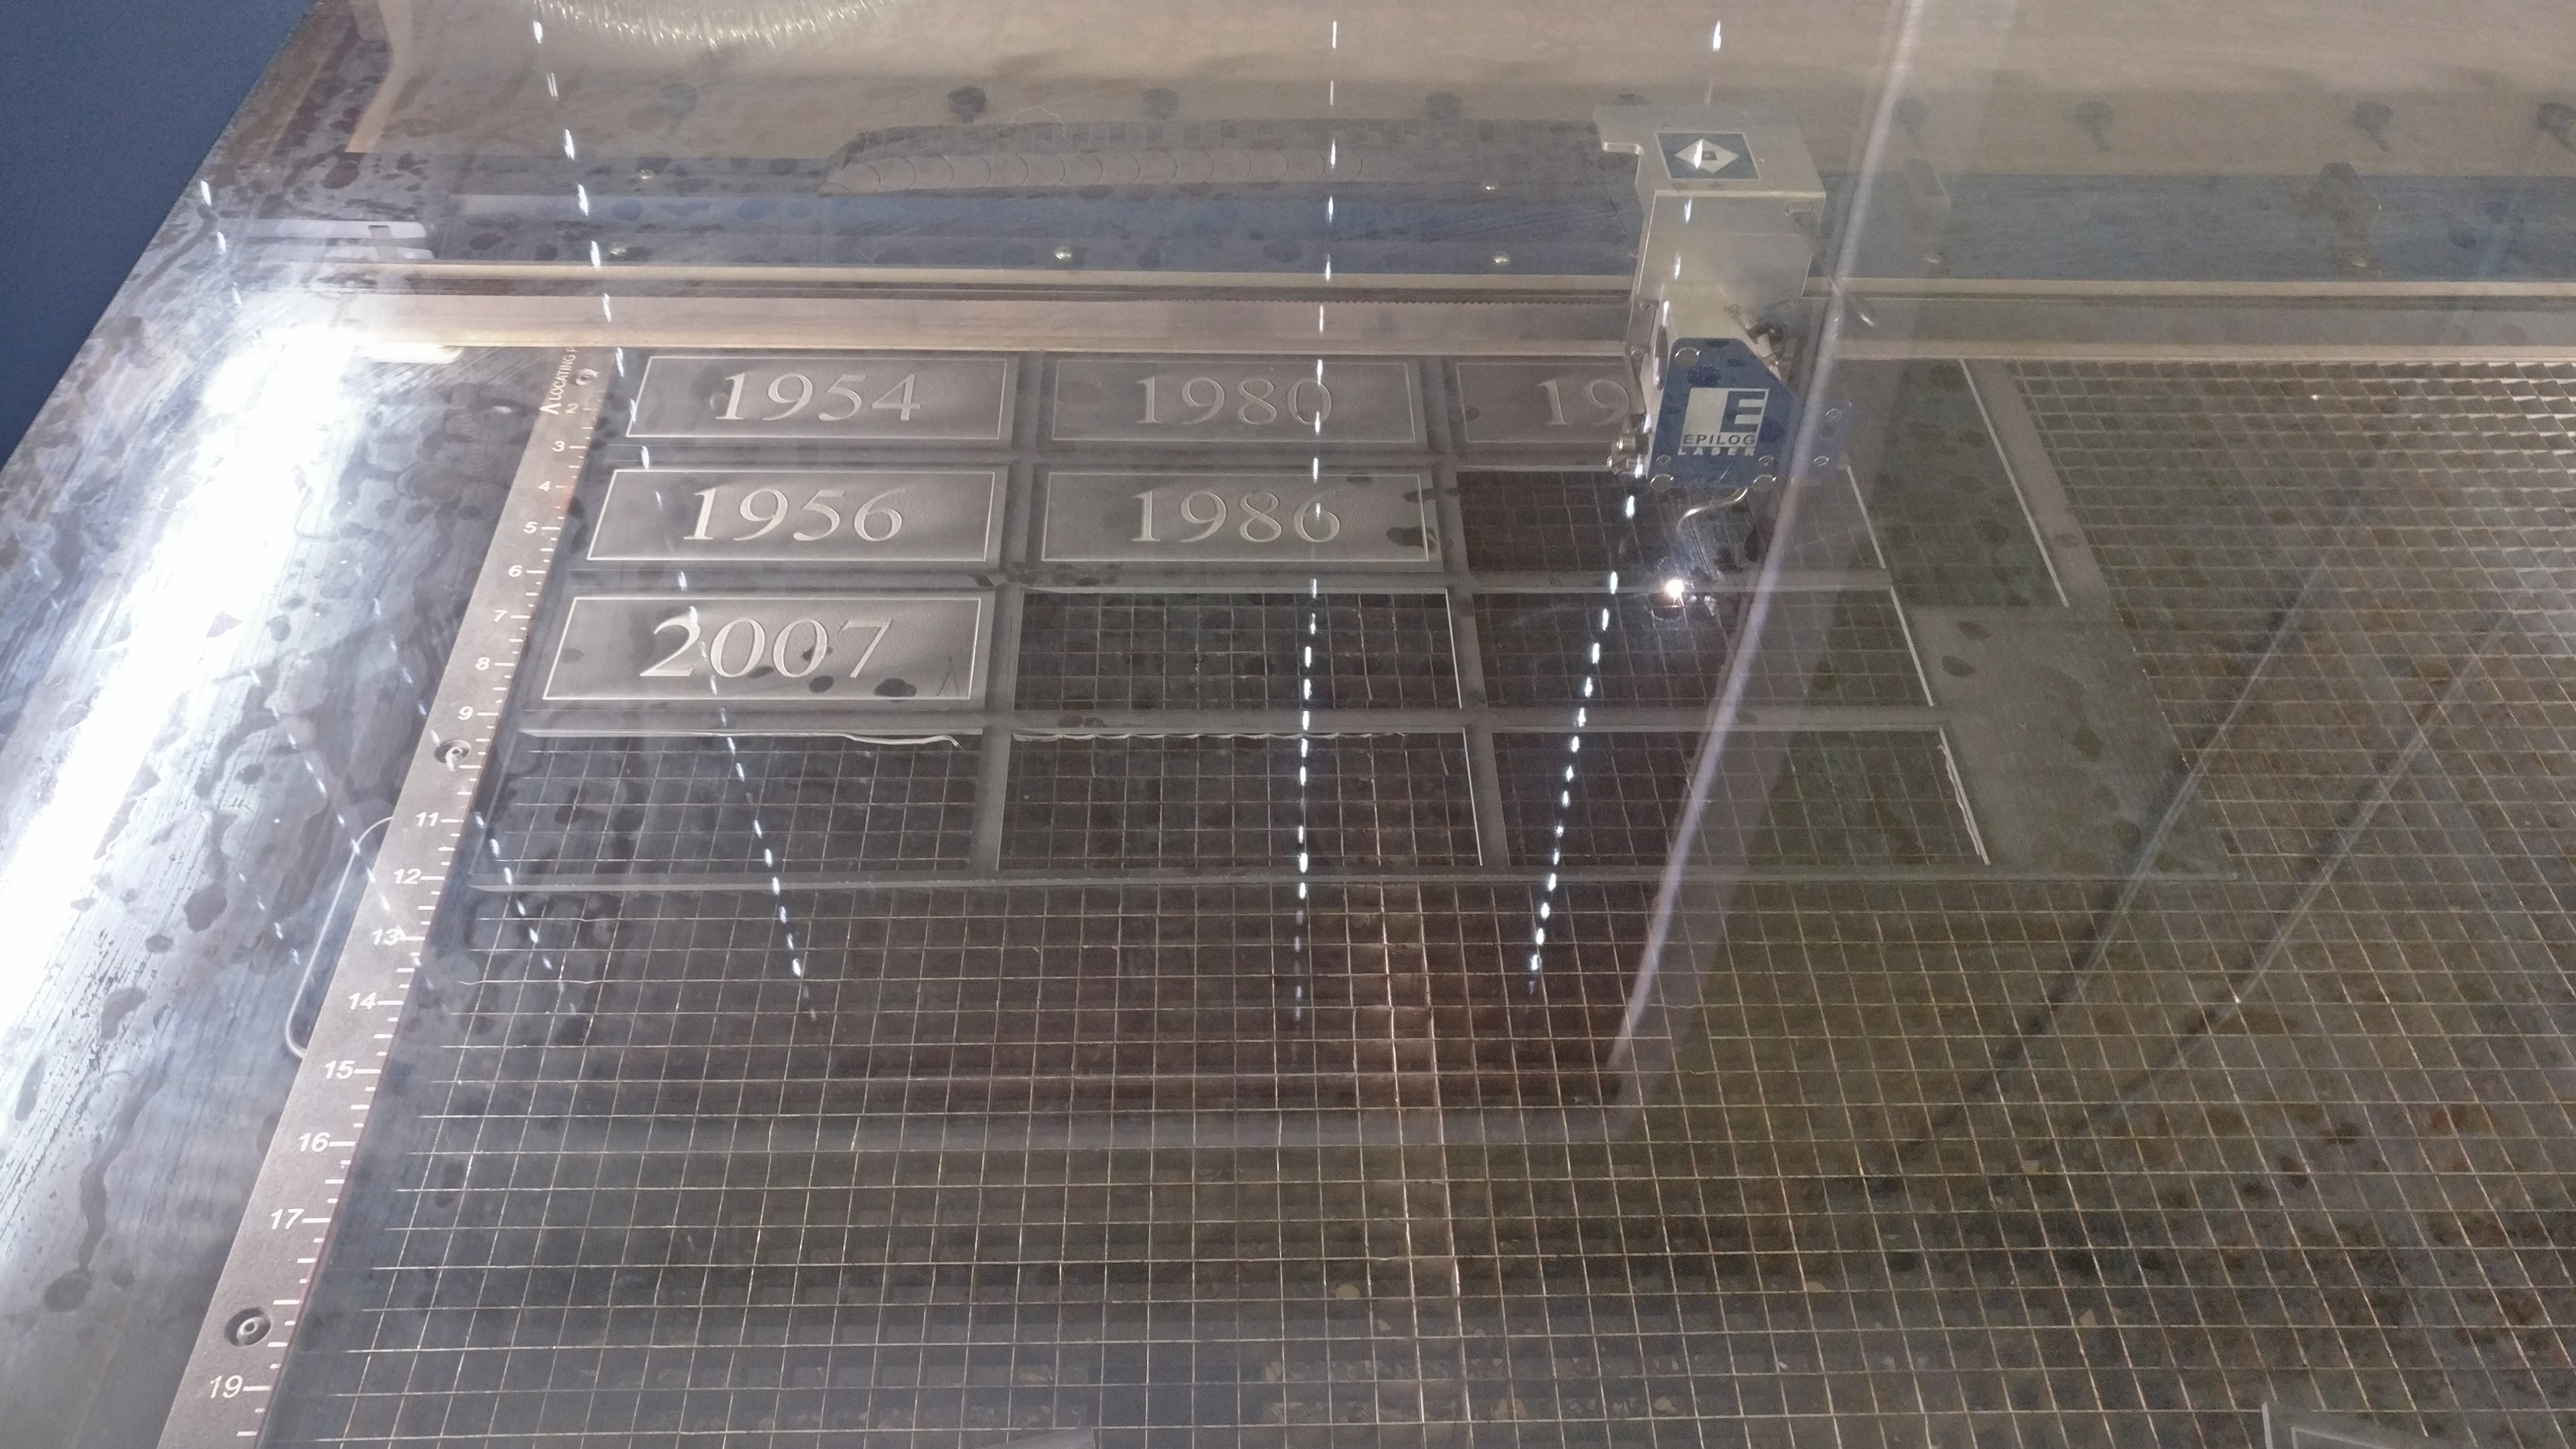
\includegraphics[width=0.48\textwidth]{../99_Bilder/laser.jpg} & 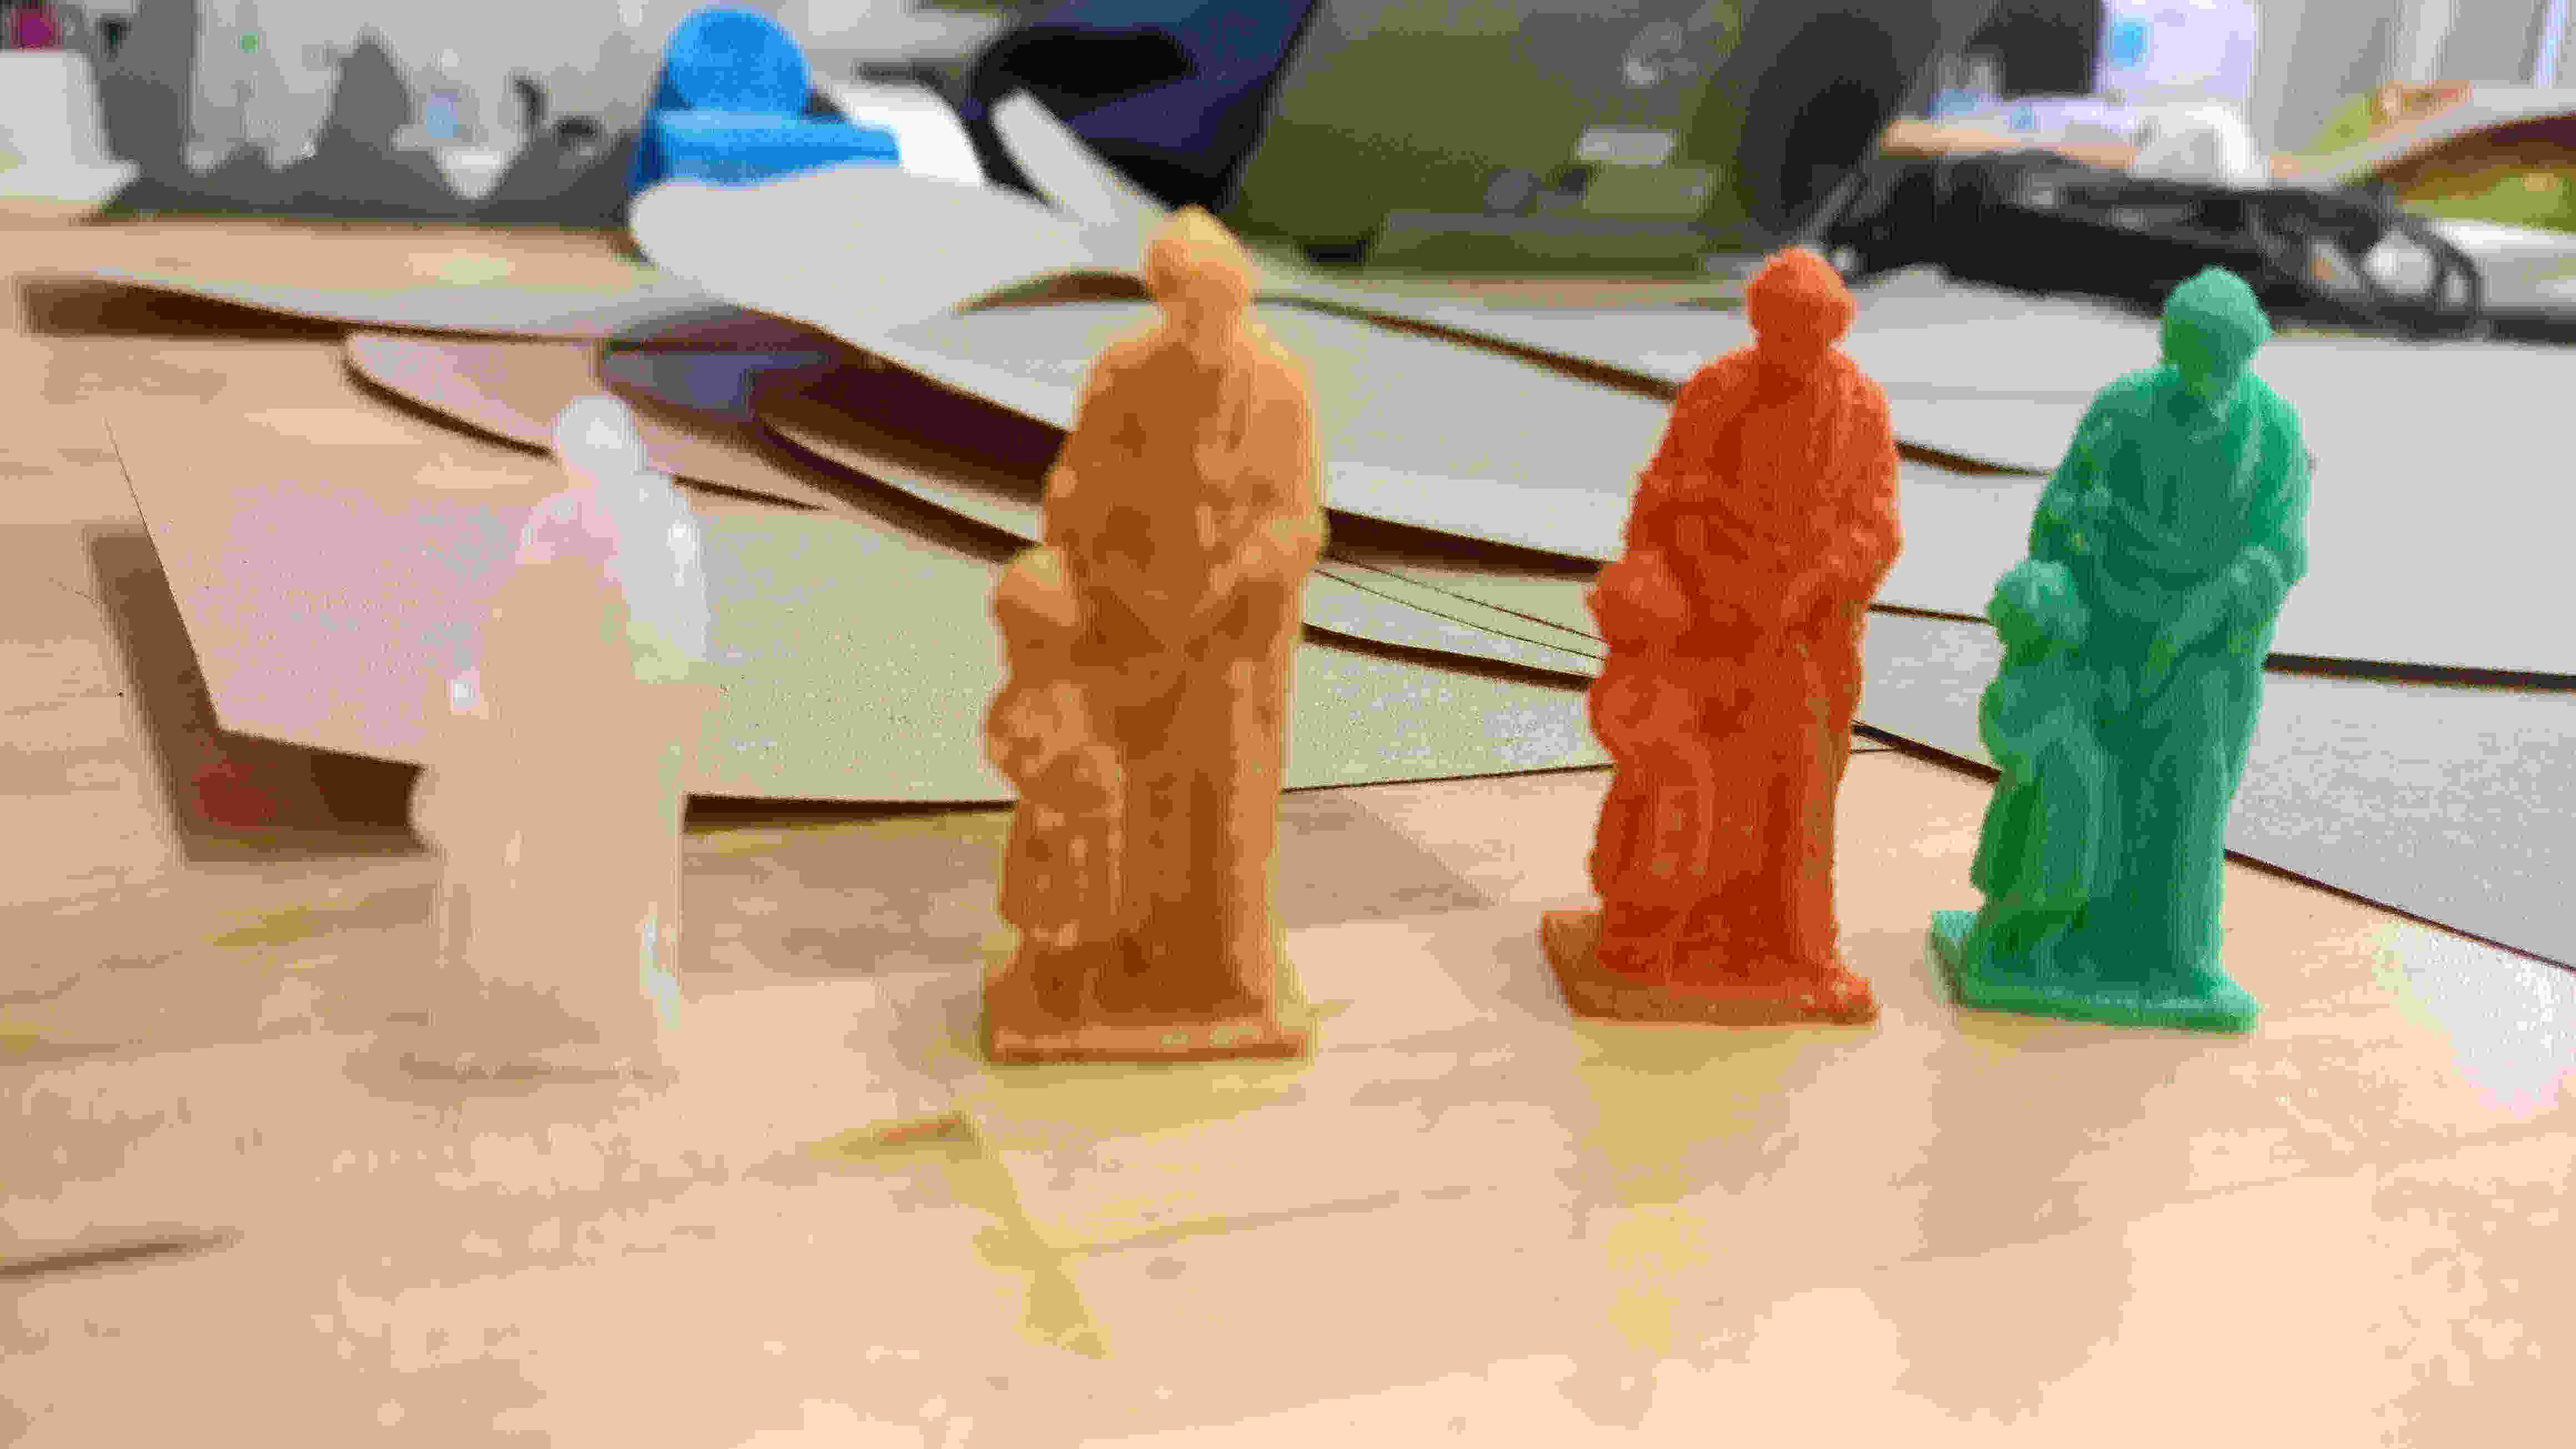
\includegraphics[width=0.48\textwidth]{../99_Bilder/3DPrint.jpg}
			\end{tabularx}
		\end{center}
		Das Prinzip des fächerübergreifenden Unterrichts wird besonders in diesem Bereich sehr stark gelebt und angewendet.
		\section{Helpdesk}
		Im Rahmen einer 1999 angelegten Kooperation mit Hewlett-Packard erhielt damals und erhält auch heute noch jede Schülerin einen eigenen Laptop, den sie in der Schule wie auch privat nutzen darf. Auf dem für jede Schülerin personalisierten Laptop sind die für den Unterricht relevanten Programme installiert und alle relevanten Einstellungen getätigt bevor sie den Laptop erhält.\\
		Um die Kosten bezüglich der Wartung gering zu halten, hat die Schule Zeit und Geld in die Ausbildung einzelner Lehrkräfte investiert um sie zu zertifizierten Ausbildern zu machen.\\
		Diese Zertifizierung nutzt die Schule nun, um ihre Schülerinnen innerhalb des Helpdesks selbst zu zertifizierten Angestellten auszubilden. Hierfür lernen die Schülerinnen zum einen die einzelnen Hard- und Software-Komponenten und werden darin trainiert, die Schul-Laptops auf Fehler zu analysieren, diese gegebenenfalls softwareseitig zu beheben und andernfalls die Rechner auseinander zu bauen und defekte Teile auszutauschen.\\
		\begin{center}
			\begin{tabularx}{\textwidth}{XX}
				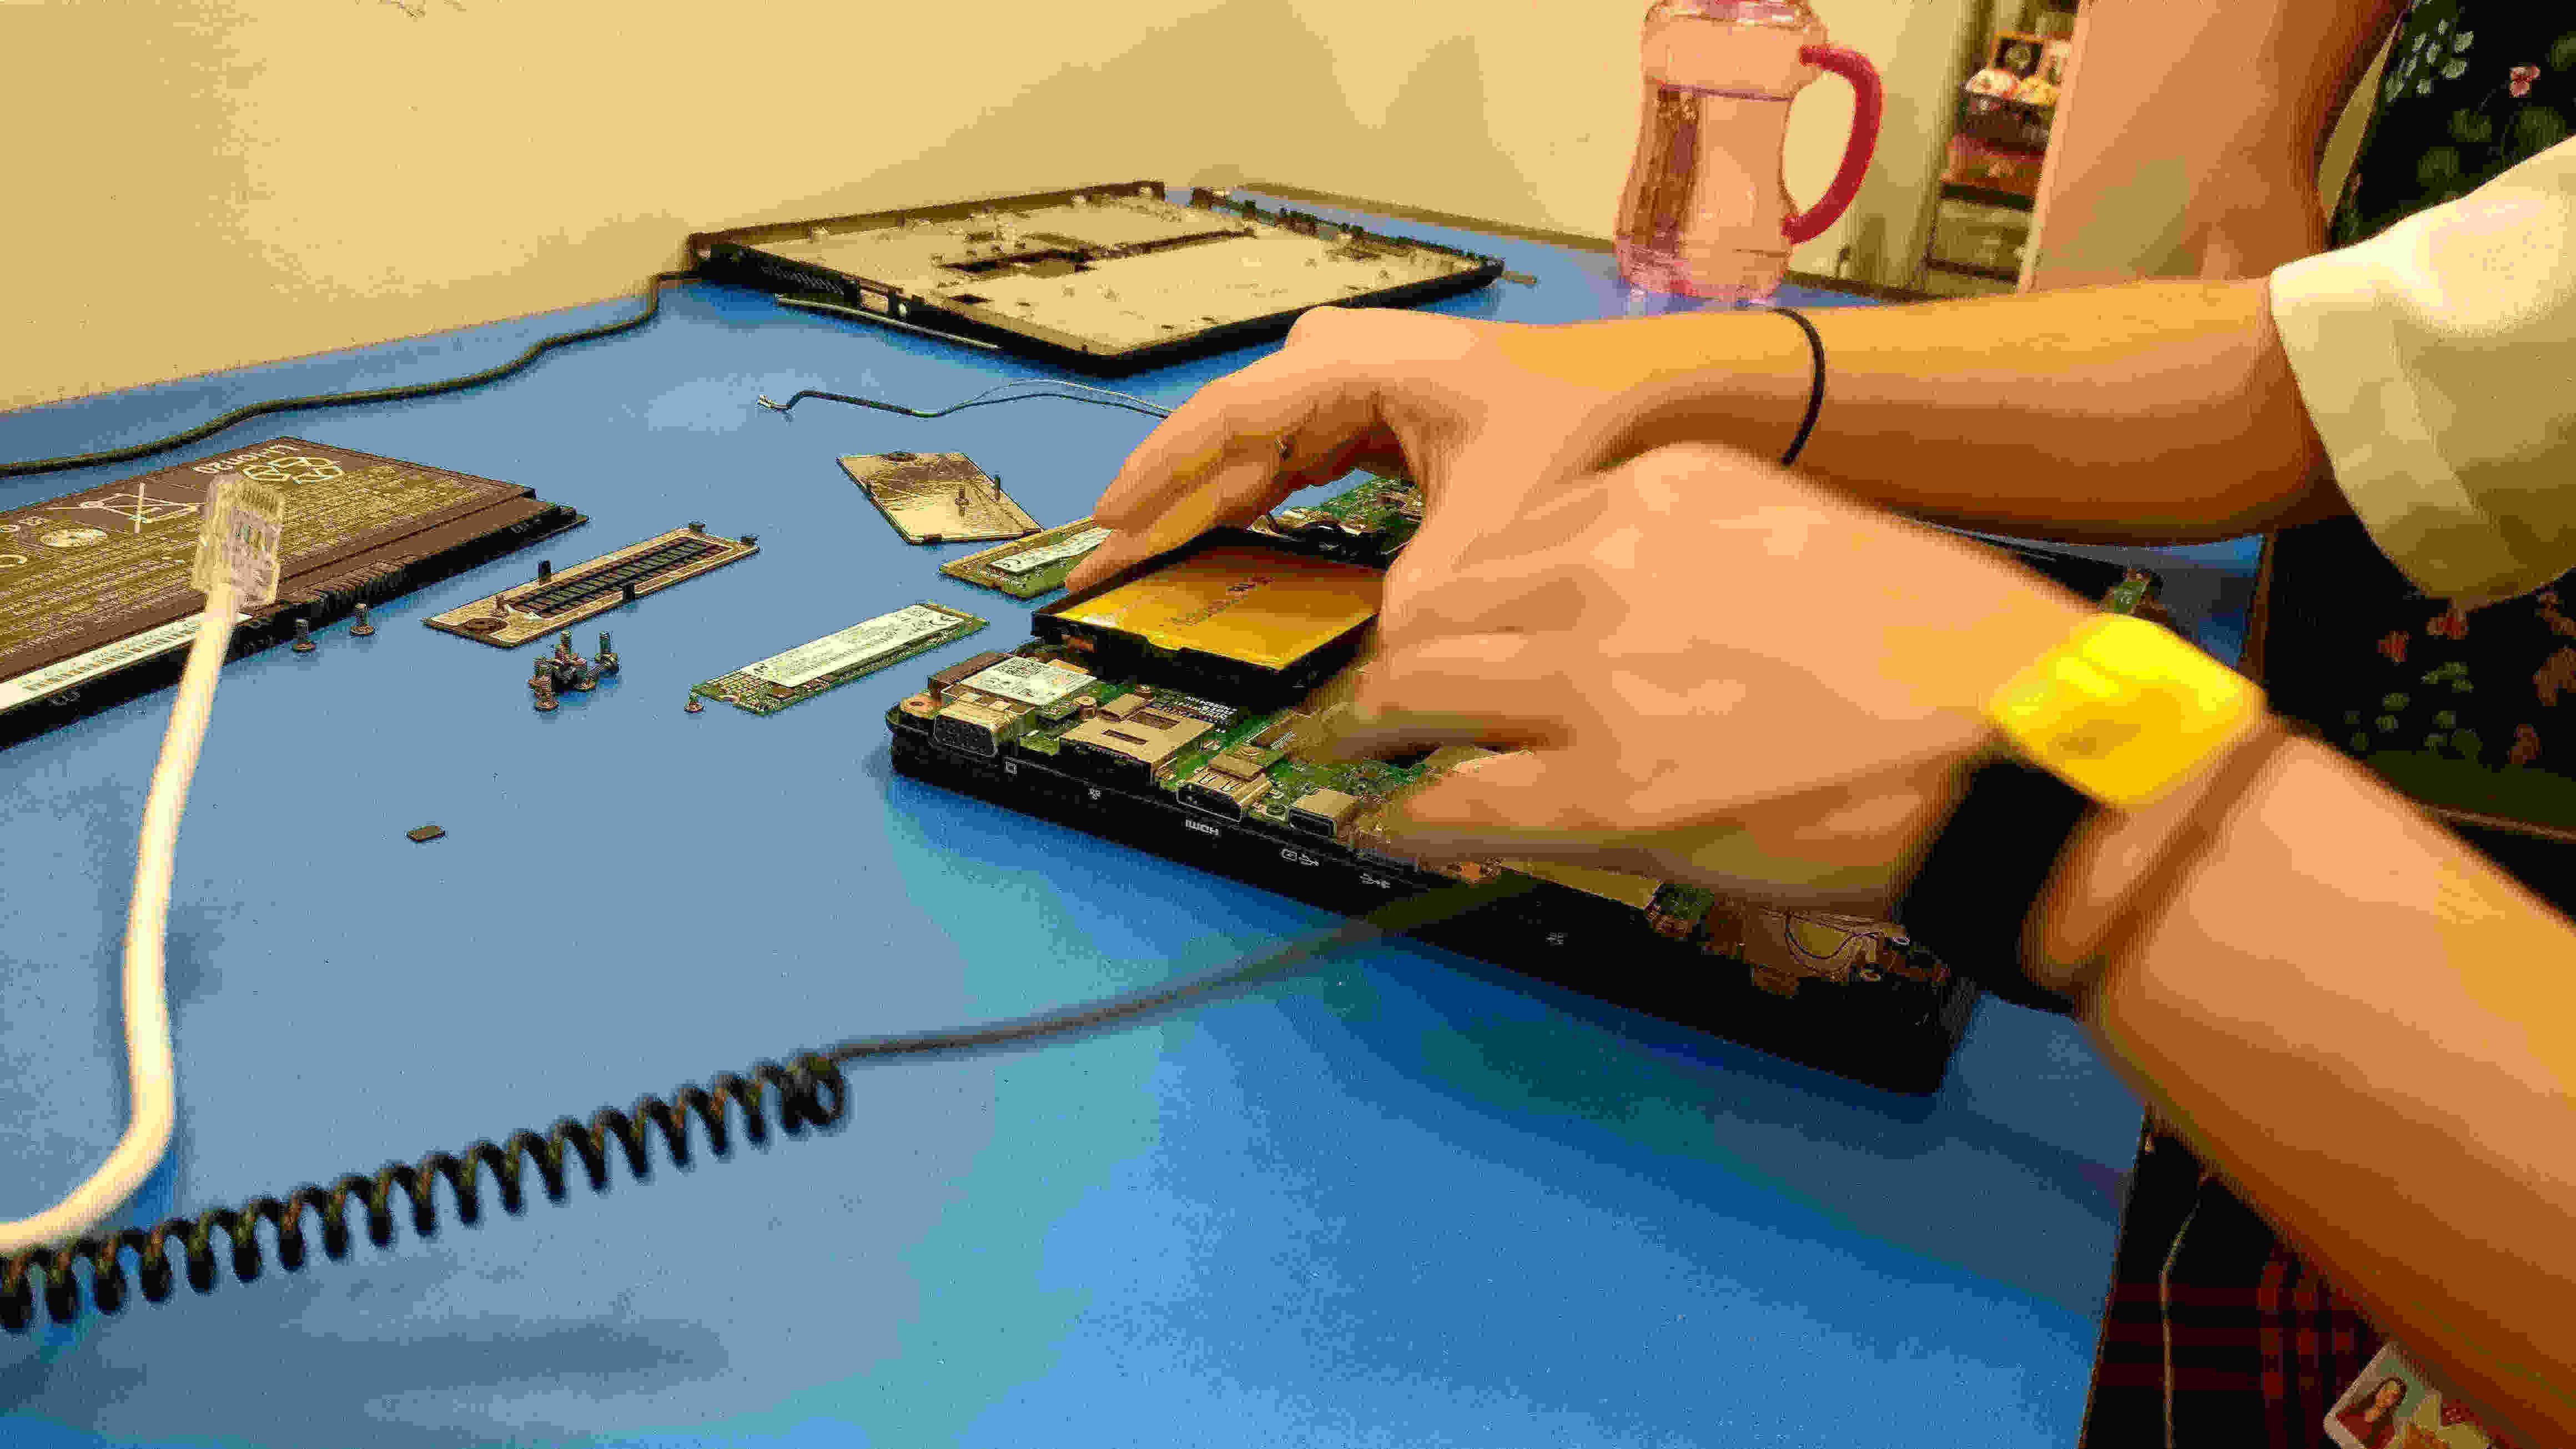
\includegraphics[width=0.48\textwidth]{../99_Bilder/00_HD.jpg} & 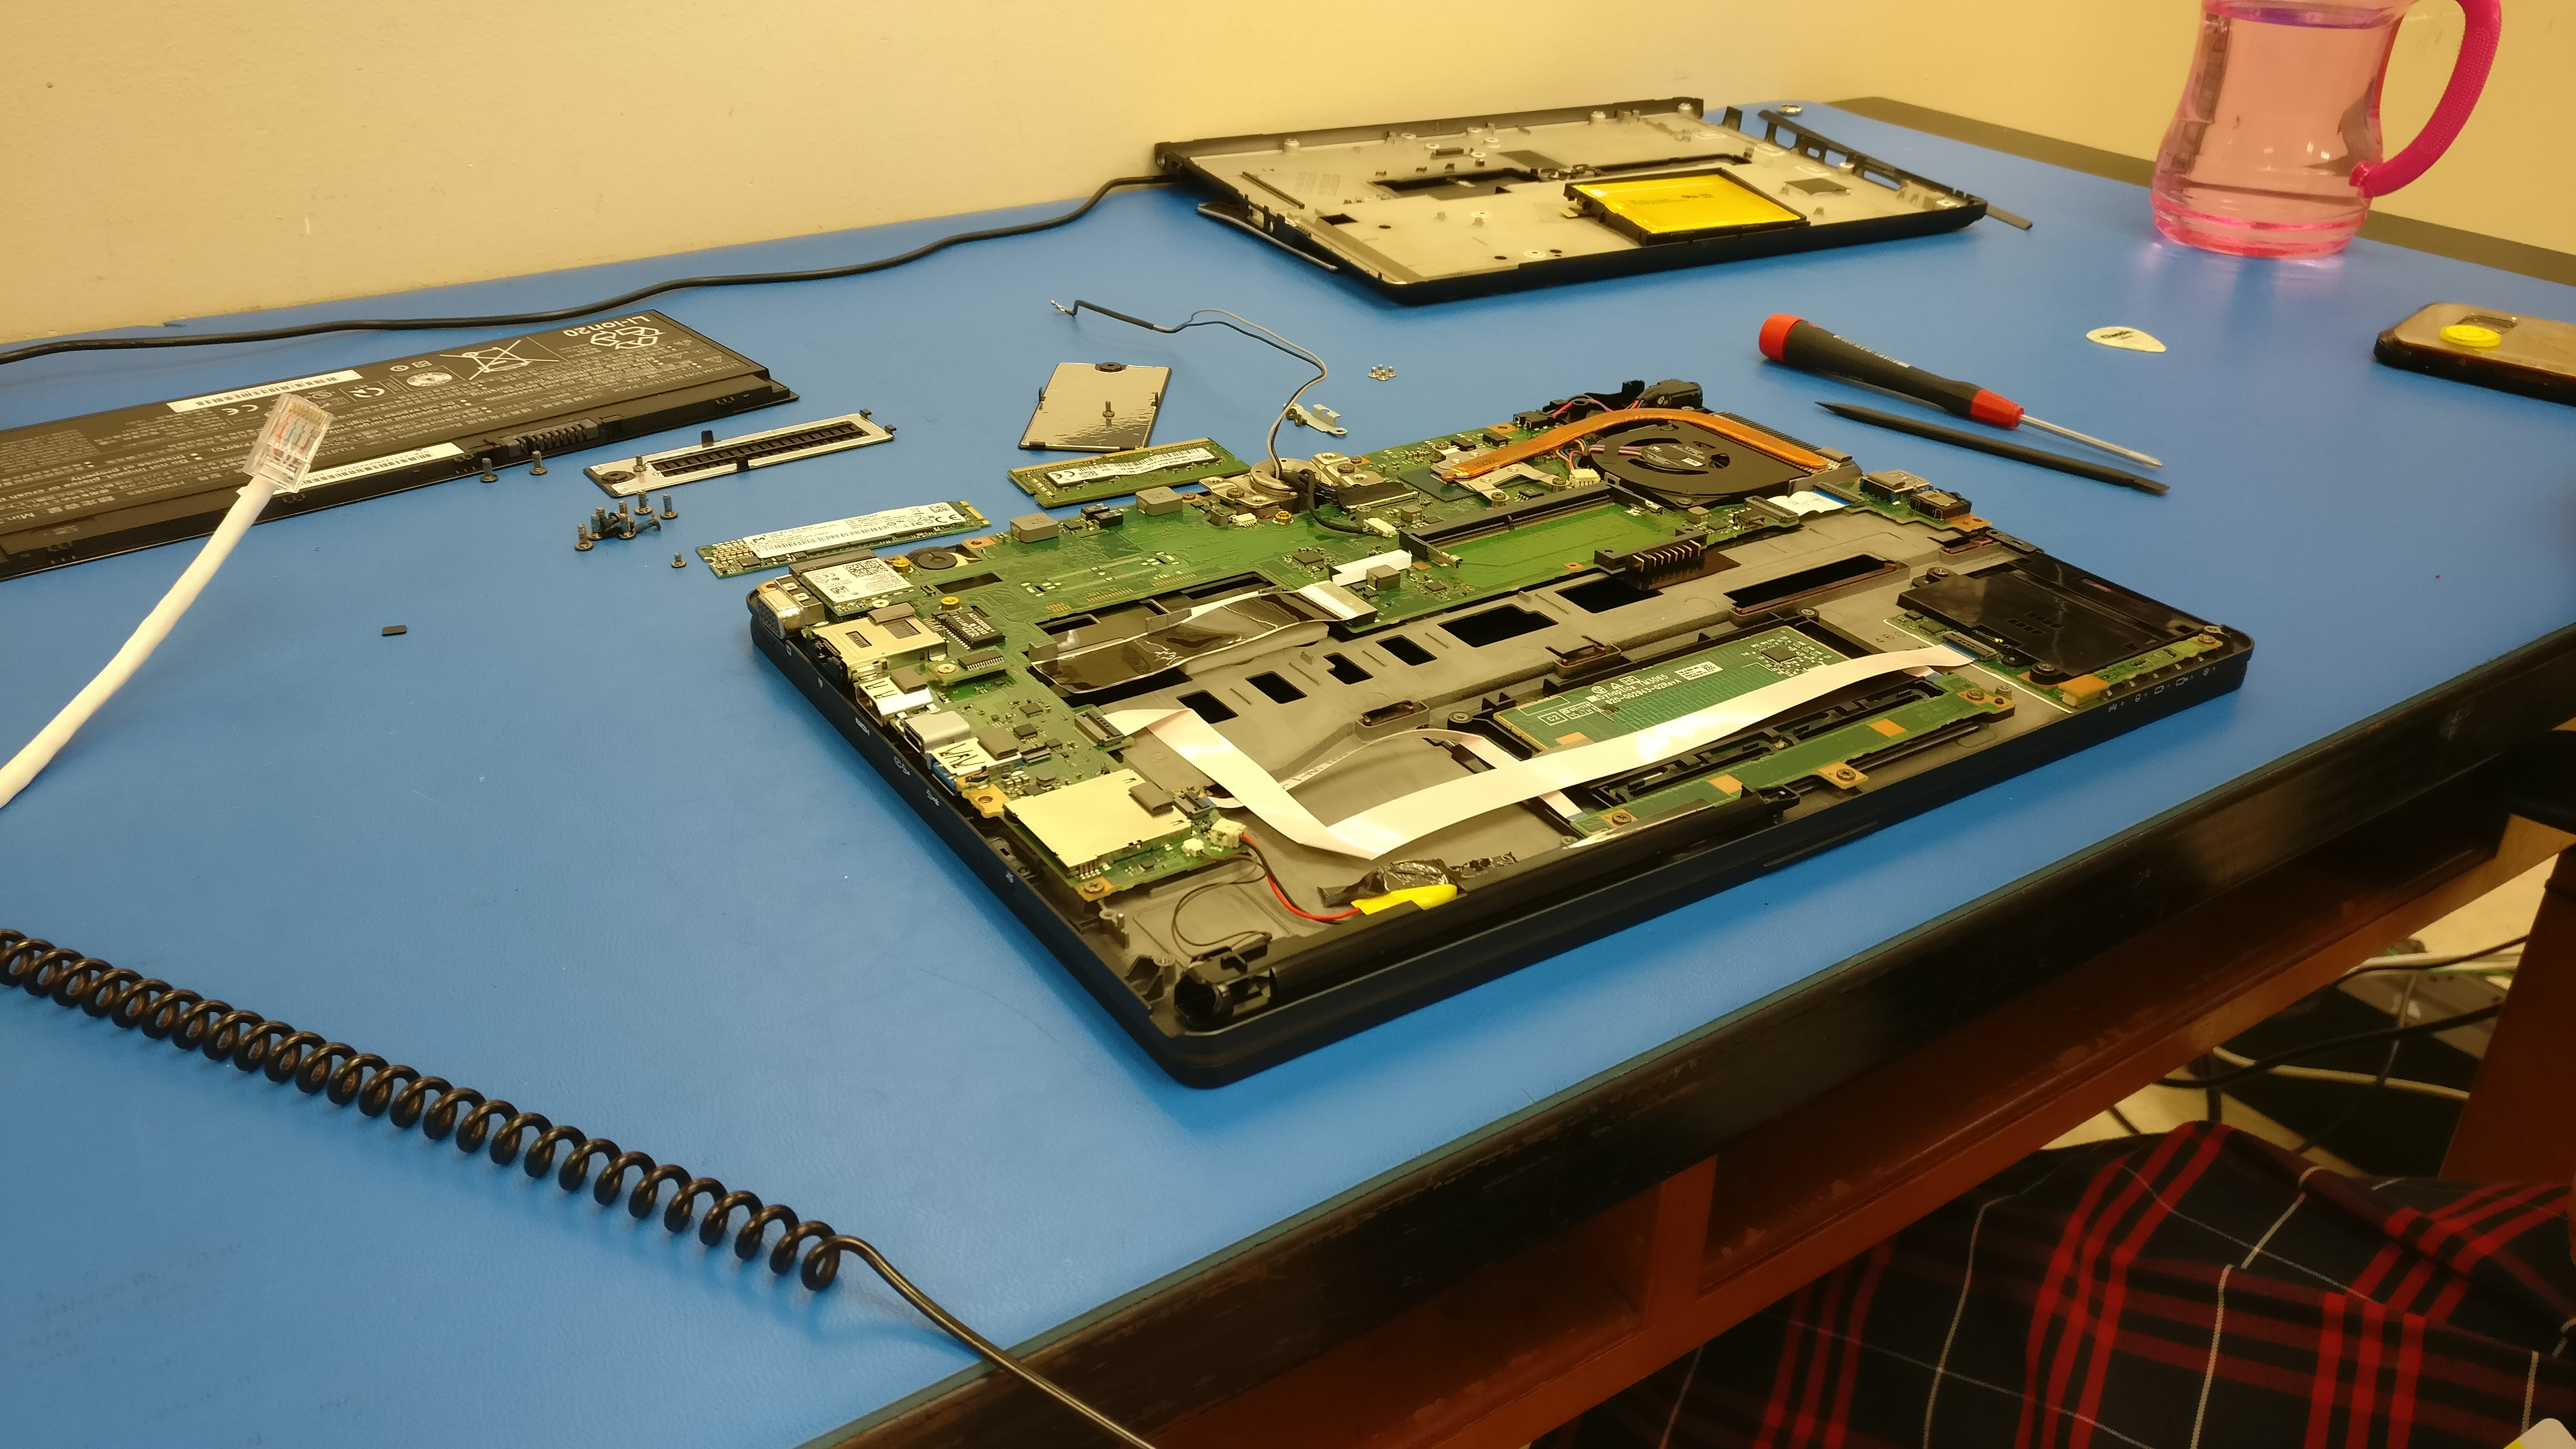
\includegraphics[width=0.48\textwidth]{../99_Bilder/01_HD.jpg}
			\end{tabularx}
		\end{center}
		Dieses Konzept stärkt nicht nur das Selbstvertrauen der Schülerinnen in sich selbst und in ihre Fähigkeiten. Es unterstützt die Schülerinnen zudem dabei ihre Leidenschaft bzw. Begeisterung für die Arbeit mit Hard- und Software zu entdecken und auszuleben.\\
		Zudem erhalten die Schülerinnen bereits in der Schule eine qualifizierende Ausbildung sowie ein offizielles Zertifikat, welches ihnen den Einstieg in das Berufsleben deutlich erleichtert.\\
		\par\noindent
		Ein ähnliches Konzept würde sich besonders in den Höheren Berufsfachschulen mit der Fachrichtung IT in der Oberstufe anbieten. Zusätzlich zu dem obligatorischen Praktikum könnten die die Schüler hier während der Schulzeit Praxiserfahrung sammeln können und an realen Problemen arbeiten.
		\subsection{Memorable Impressions}
		Sicherlich habe ich die meiste Zeit in der Schule verbracht. Dennoch habe ich es an meinem ersten Samstag, dem 01.10.2018, geschafft ein LSU Football Game zu besuchen.\\
		Ich bin nicht groß Sport-begeistert, aber dieses Gefühl und die Begeisterung der Menge im Stadion war einfach nur mitreißend.\\
		\begin{center}
			\begin{tabularx}{\textwidth}{XX}
				\includegraphics[width=0.45\textwidth]{../99_Bilder/00_LSU.jpg} & \includegraphics[width=0.45\textwidth]{../99_Bilder/01_LSU.jpg}
			\end{tabularx}
		\end{center}
		Am Tag vor meiner Abreise habe ich noch einen Ausflug nach New Orleans gemacht. Der imposante Stadtkern und die schönen alten Fassaden der Häuser spiegeln den Südstaaten-Flair richtiggehend wieder.\\
		\begin{center}
			\begin{tabularx}{\textwidth}{XX}
				
\includegraphics[width=0.45\textwidth]{../99_Bilder/00_trip.jpg} & 
\includegraphics[width=0.45\textwidth]{../99_Bilder/01_trip.jpg} 
			\end{tabularx}
		\end{center}
		An jeder Straßenecke werden die \textit{Louisiana Oyster} angepriesen, so dass ich nicht darum herum gekommen bin mich sowohl kulturell wie auch kulinarisch weiterzubilden.\\
		\begin{center}
			\begin{tabularx}{\textwidth}{XX}
				
\includegraphics[width=0.45\textwidth]{../99_Bilder/00_food.jpg} & 
\includegraphics[width=0.45\textwidth]{../99_Bilder/01_food.jpg}
			\end{tabularx}
		\end{center}
		\section{Fazit}
		Als besonders wertvoll und für meine eigenes weiteres Handeln prägend sehe ich meine Beobachtung, dass eine persönliche Beziehung und ein gewisses Interesse der Lehrperson an der Freizeit und den privaten Interessen der Schüler für das Arbeitsklima und die Motivation der Schüler förderlich sein kann.\\
		\textit{Ich persönlich würde aber nicht so weit gehen, wie die Lehrkräfte an der SJA, und den Schülern gestatten, mich mit dem Vornamen anzusprechen. Dieser Ausspruch "}Frau Wesp...\textit{" ist für mich wichtig, um die nötige Objektivität bezüglich der Schülerleistungen zu wahren.}
		Zudem habe ich beobachten können, dass sich die Schüler eher um Hilfe zu bitten, wenn sie Vertrauen zur Lehrkraft haben und diese im Allgemeinen Wertschätzend mit den Schülern umgeht.\\
		Ich werde also versuchen, eine persönlichere aber dennoch auf Distanz basierte Beziehung zu führen um sie so in ihrem Lernerfolg besser unterstützen zu können.\\
		\par\noindent
	\end{worksheet}
\end{document}